%%%%%%%%%%%%%%%%%%%%%%%%%%%%%%%%%%%%%%%%%%%%%%%%%%%%%%%%%%%%%%%%%%%%%%%
%
% Presentation of Beamer UMN Theme
% Beamer Presentation by Tambe E. Norbert of UMN--Twin Cities
% Hacked From Chris Bourke of Univ Nebraska--Lincoln
% June 13th, 2014
%
%%%%%%%%%%%%%%%%%%%%%%%%%%%%%%%%%%%%%%%%%%%%%%%%%%%%%%%%%%%%%%%%%%%%%%%
\documentclass{beamer}
\usetheme[hideothersubsections,hideallsubsections]{UMNTheme}
\newcommand {\framedgraphic}[2] {
    \begin{frame}{#1}
        \begin{center}
            \includegraphics[width=\textwidth,height=0.8\textheight,keepaspectratio]{#2}
        \end{center}
    \end{frame}
}
% Remove navigation symbols
\setbeamertemplate{navigation symbols}{}
\title{Search For Long-Lived Neutral Particles Decaying To Photons In CMS}
\subtitle{PhD Oral Exam}
%\vspace{-5cm}
\author[Tambe E. Norbert]{Tambe E. Norbert \\ University Of Minnesota} % (optional, for multiple authors)
%{Shih-Chuan Kao\inst{1} \and Yuichi Kubota\inst{1} \and Tambe E. Norbert\inst{1} \and Roger Rusack\inst{1}}
%\institute[UMN]{ \inst{1} University Of Minnesota}
\vspace{-20cm}
%\date{ Long-Lived Meeting,\\ \today}
\date{ \\ \today}

\begin{document}
%{% open a Local TeX Group
%\setbeamertemplate{sidebar}{}
\begin{frame}
\titlepage
\begin{center}
\href{mailto:norbe072@umn.edu}{\color{cyan}{\texttt{norbert@physics.umn.edu.edu}}}
\end{center}
\end{frame}




\section*{MENU}
{
\usebackgroundtemplate{%
\tikz\node[opacity=0.3] {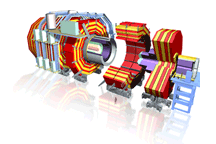
\includegraphics[height=\paperheight,width=\paperwidth]{/home/tensr/Documents/TEN-HEP-PHD-THESIS/PHD_THESIS/PHD/PLOTS/CMS_DET.png}};}
\begin{frame}
\frametitle{\huge{MENU}}
\tableofcontents
\end{frame}
}
%%% Intro to Talk
\section{INTRODUCTION}

{
\usebackgroundtemplate{%
\tikz\node[opacity=0.35] {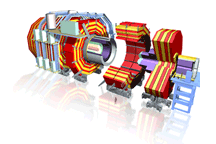
\includegraphics[height=\paperheight,width=\paperwidth]{/home/tensr/Documents/TEN-HEP-PHD-THESIS/PHD_THESIS/PHD/PLOTS/CMS_DET.png}};}
\begin{frame}
  \begin{center}
   \textcolor{UMN@Maroon}{\Huge{\textbf{INTRODUCTION}}}
  \end{center}
\end{frame}
}

\begin{frame}
\frametitle{\Huge{Modern Particle Physics}}
 \begin{minipage}[t]{\paperwidth}
% \begin{columns}
  % \begin{column}{0.70\linewidth} 
     % \begin{itemize}
     \mbox{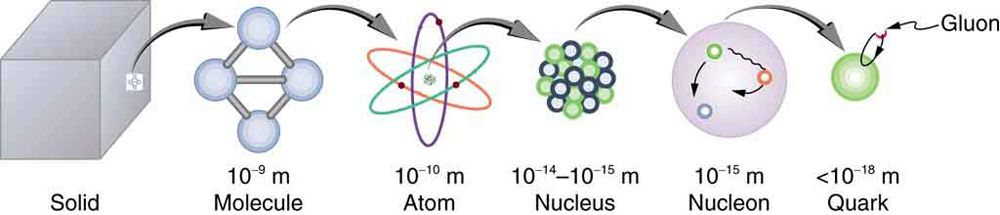
\includegraphics[height=0.50\paperwidth, width=0.85\paperwidth]{THESISPLOTS/New-Physics-PLOTS/Matter-Content-Particle-Physics.jpg}}
       %\item \textbf{Particle Physics}: physics of \textcolor{red}{very small} and  \textbf{Cosmology}: physics of \textcolor{blue}{very large}
     % \end{itemize}
    % best describes the universe with \textcolor{UMN@Maroon}{\textbf{unprecedented precision}}.
    % Studying particle properties like,
    % \begin{itemize}
    %   \item Mass, Charge, Magnetic Moment, Spin, and \textcolor{UMN@Maroon}{\textbf{Lifetime}}.
    % \end{itemize}   
    % Particle Classification table of our universe.  
   % \end{column}
  % \begin{column}{0.45\linewidth}
    %\mbox{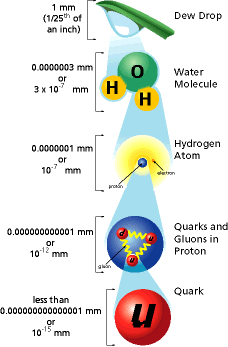
\includegraphics[height=0.55\textwidth, width=0.75\linewidth]{THESISPLOTS/New-Physics-PLOTS/Matter_Building_Blocks.png}}
 %The \textcolor{UMN@Maroon}{\textbf{Standard Model}}  
    %\vspace{0.5cm}
    
 %  \end{column}
% \end{columns}

\vspace{1cm}
 \textcolor{blue}{\textbf{Matter at lengths from $10^{-18}$~m to $10^{26}$~m}}
 
 \end{minipage}

\end{frame}

% The Standard Model
\begin{frame}
\frametitle{\Huge{Standard Model Recipe}}
\centering
 \mbox{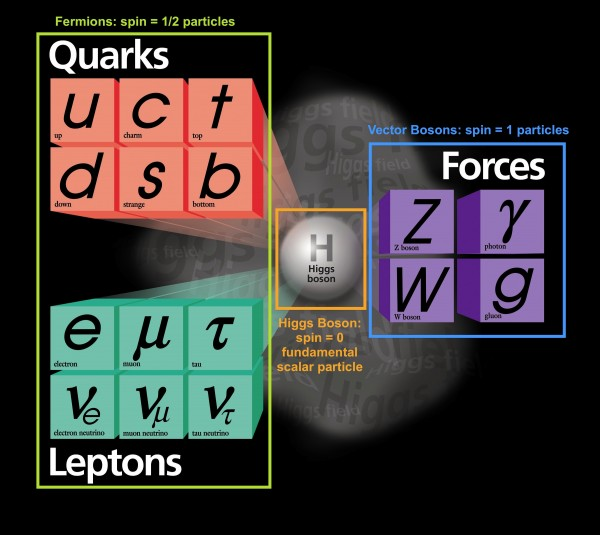
\includegraphics[height=0.40\textwidth, width=0.75\linewidth]{THESISPLOTS/FULL-SM-P.jpg}}
\begin{minipage}[b]{0.95\paperwidth}
    \begin{columns}
      \begin{column}{0.60\paperwidth}
       \begin{itemize}
       \item \textcolor{UMN@Maroon}{\textbf{\huge{Reality Recipe}}}
         \begin{itemize}
         \huge{
          \item 6 quarks and leptons,
          \item 4 force mediators,
          \item 1 Higgs Boson.
          }
           %\item Forceful spices not a single spice?
           %\item Recipe can also prepare Dark Matter?
           %\item Is this list of ingredients complete?
           %\item Origin of these ingredients?
         \end{itemize}
        \end{itemize}
      \end{column}   
      \begin{column}{0.45\paperwidth}
      \mbox{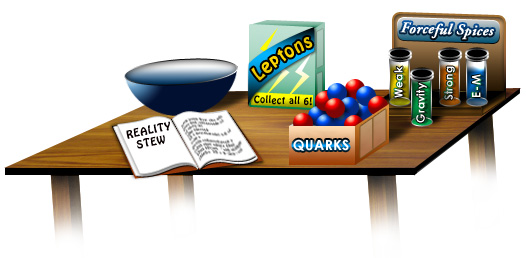
\includegraphics[height=0.85\textwidth, width=0.70\linewidth]{THESISPLOTS/New-Physics-PLOTS/Reality_Recipe_stew.jpg}}
      \end{column}      
     \end{columns}   
 \end{minipage}
 
\end{frame}

%% The Universe Budget
\begin{frame}
\frametitle{\Huge{The Universe}}
 \begin{minipage}[t]{\paperwidth}
    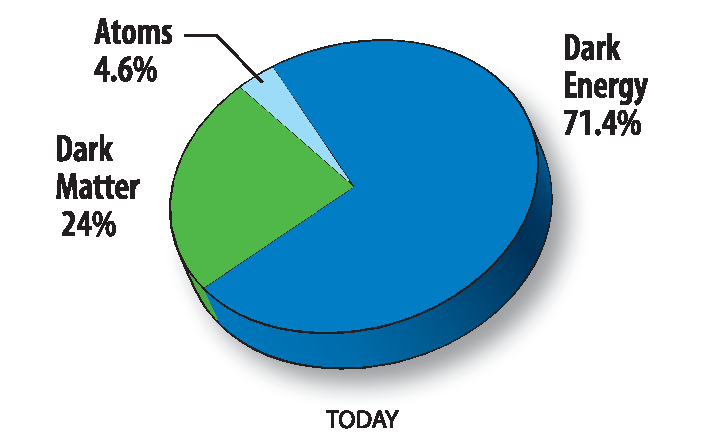
\includegraphics[height=0.60\paperwidth,width=0.85\paperwidth]{THESISPLOTS/WMAPUniversePie.pdf}    
 \end{minipage}
  \vspace{-0.09cm}
 \textcolor{UMN@Maroon}{\textbf{What are the fundamental constituents of the Universe?}}
\end{frame}



%% New Physics Theory
\begin{frame}
\frametitle{\Huge{Past, Present, Future}}
%\textbf{Still expecting New Physics?}
  %\begin{columns}
  \begin{minipage}[b]{0.65\paperwidth}
    %\begin{multicols}{2}
     \begin{varblock}[6.5cm]{\textbf{\huge{The Universe  Spin Set}}}
     \huge{
       $S =\Big\{\textcolor{blue}{\mathbf{0}}, \frac{1}{2}, 1,  \frac{3}{2}, 2  \cdots \Big\} \hbar $ 
       }
     \end{varblock}
     %\columnbreak
     %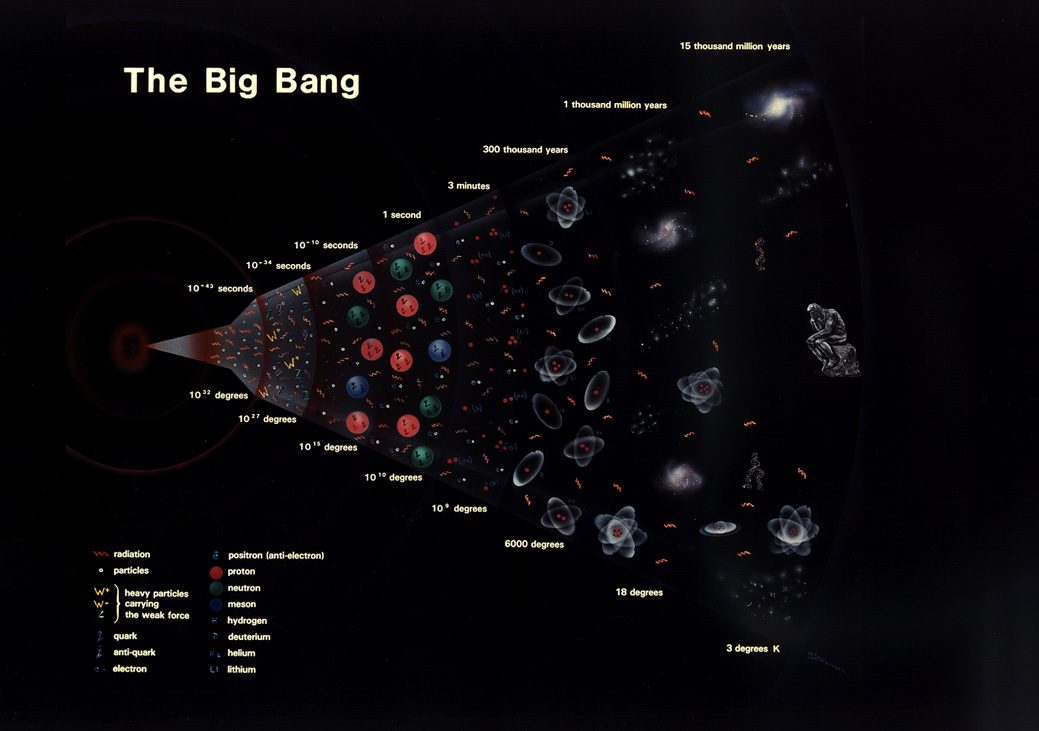
\includegraphics[height=0.45\textwidth,width=0.40\paperwidth]{THESISPLOTS/New-Physics-PLOTS/Big_Bang.jpg}
 %\end{multicols}
 \end{minipage}
\begin{minipage}[b]{0.70\paperwidth}
%Our current understanding:
 \begin{columns}
    \begin{column}{0.65\linewidth} 
     \begin{itemize}
     \item $\mathbf{s = \frac{1}{2}\hbar}$ Describes all the matter in our universe.
     \item $\mathbf{s = 1\hbar}$ Describes gauge interactions.
     \item $\mathbf{s = \textcolor{blue}{0}\hbar}$ Responsible for mass.
     \item $\mathbf{s = 2\hbar}$ Describes gravity~(gauged?).
    
    \end{itemize}
    This \textit{Spin} set describes  only $\approx 4.6$\% of our total universe.
   \end{column}
     \begin{column}{0.45\linewidth}
      \begin{itemize}
       \item $\mathbf{s = \frac{3}{2}\hbar}$ \textcolor{red}{?? \textbf{Dark Matter}?}
      \end{itemize}
    \mbox{
    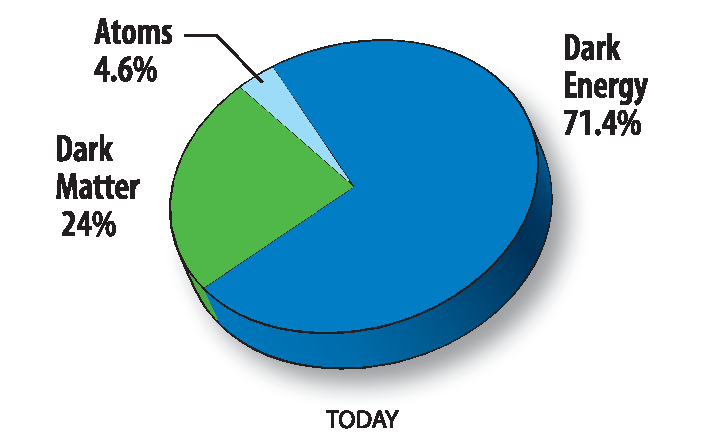
\includegraphics[height=0.65\textwidth,width=0.45\paperwidth]      {THESISPLOTS/WMAPUniversePie.pdf}}
    \end{column}
\end{columns}
\end{minipage}
\end{frame}

\begin{frame}
\frametitle{\Huge{Supersymmetry}}
\begin{minipage}[t]{\linewidth}
  \begin{columns}
    \begin{column}{0.6\textwidth}
Supersymmetry(SUSY) allows for \\
 \textbf{Bosons} $ \mathrel{\overset{\makebox[0pt]{\mbox{\normalfont\tiny SUSY}}}{\Longleftrightarrow}} $ \textbf{Fermions}.
\begin{align*}
 \mathsf{Q}\Ket{\mathbf{Bosons}} &= \Ket{\mathbf{Fermions}} 
 \end{align*}
 \begin{align*}
 \mathsf{Q}\Ket{ \mathbf{Fermions}} &= \Ket{\mathbf{Bosons}}
 \end{align*}
 
    \end{column}
    \begin{column}{0.4\textwidth}
     \mbox{
    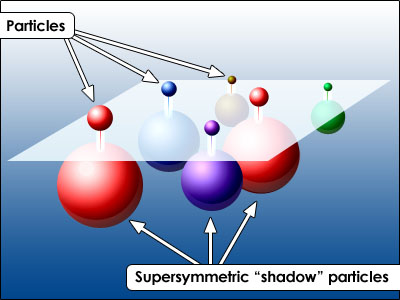
\includegraphics[height=0.65\textwidth,width=0.30\paperwidth]{THESISPLOTS/New-Physics-PLOTS/sypersymmetry.jpg}}
    \end{column}
 \end{columns}    

\end{minipage}
\begin{minipage}[t]{\linewidth}
  \begin{varblock}[7cm]{\textbf{Supersymetry Motivation}}
  \begin{itemize}
   \item Allows for unification of fundamental forces,
   \item Natural frame work for unifying Gravity and Quantum Mechanics,
   \item Stabilizes the Higgs mass and explains energy scale hierarchy,
   \item \textcolor{UMN@Maroon}{\textbf{Predicts long-lived neutral and stable particles which could describe Dark Matter}}.
  \end{itemize}
  \end{varblock}
\end{minipage}
\end{frame}

\begin{frame}
\frametitle{\Huge{Interaction  Life Time}}
\end{frame}



%% Motivation for Long-Lived Particle Search
\begin{frame}
\frametitle{\Huge{Long-Lived Particles}}
 %\vspace{-0.5cm}
\begin{minipage}{0.85\paperwidth} 
     %\begin{itemize}  
       %\item{\color{UMN@Maroon} \textbf{\huge{ Gauge Mediated Supersymetry Breaking models}}}     
      %% \setbeamertemplate{itemize items}{$\mathbb{\star}$}
       % %\begin{itemize}
        % %\item{\color{UMN@Maroon} \textbf{\huge{GMSB Models}}}
       \textcolor{UMN@Maroon}{\textbf{\huge{GMSB Models}}}
         %\huge{Gauge Mediated Supersymmetry Breaking~(GMSB)}    
        \setbeamertemplate{itemize items}{$\mathbb{\triangleright}$}
          \begin{itemize}  
           \Large{  
            \item Next-to-lightest SUSY~(NLSP) is \alert{Neutralino}~($\tilde{\chi}^{0}_{1}$),
            \item $eV-keV$ mass Lightest-SUSY particle~(LSP) is \textcolor{blue}{Gravitino}~($\tilde{G}$),
            \item Gravitino is a Dark Matter Candidate.
           }
          \end{itemize}
       % \setbeamertemplate{itemize items}{$\mathbb{\star}$}  
       % \item General Gauge Mediation~(GGM)
       %  \setbeamertemplate{itemize items}{$\mathbb{\triangleright}$}
       %   \begin{itemize}
        %    \item NLSP is a mixture of fermions~(Bino, Wino, Higssino).
         %   \item Several SUSY particles can be NLSP.
        %  \end{itemize}
     %\end{itemize}  
    %\end{itemize}
   \end{minipage} 
   
%\vspace{1cm}
 
 %% \setbeamertemplate{itemize items}{$\mathbb{\star}$}
  %%\begin{itemize} 
  %%\item{ \color{UMN@Maroon} \textbf{\huge{R-Parity Conserving models}}}
  \textcolor{UMN@Maroon}{\textbf{\huge{R-Parity Conserving Models}}}   
\begin{minipage}[b]{0.90\paperwidth}
  \begin{columns}
    \begin{column}{0.50\linewidth} 
       \setbeamertemplate{itemize items}{$\mathbb{\dagger}$} %\otimes, \ominus etc
           \begin{itemize}
           \large{
             \item $\mathsf{R}$-Parity conserved, LSP is Dark Matter candidate. 
             \item Proton decay is consistent.
             \item Few Parameters.\\
             $\{ \mathbf{\Lambda},\mathbf{M}_{\mbox{mess}}, \mathbf{N}_{5}, \tan(\beta),  sgn(\mu), C_{grav} \} $ 
              
             }
           \end{itemize}                    
     \end{column}% 
     \hspace{0.5cm}
     \begin{column}{0.43\linewidth} 
              $ \mathrm{R} = (-1)^{3(B-L) + 2S} $ \\
              $\mathrm{R}\Ket{SM} = +1\Ket{SM} $ \\
              $ \mathrm{R}\Ket{SUSY}  = -1\Ket{SUSY} $ \\             
     \end{column}
   \end{columns} 
   %\vspace{0.5cm}
      
%%  \end{itemize}
\end{minipage}
\end{frame}

%% SPS8 model
\begin{frame}
\frametitle{\Huge{GMSB Model:SPS8}}
\centering
\begin{tcolorbox}[tab2,tabularx={||c|c|c|c|c|c||},title=SPS8 GMSB Model,boxrule=0.05pt]
     \bfseries{$\mathbf{M}_{\mbox{mess}} $}  & \bfseries{$\mathbf{N}_{5}$} & \bfseries{$ sgn(\mu)$}     & \bfseries{$ \tan(\beta)$}   & \bfseries{$\mathbf{\Lambda} $} & \bfseries{$ C_{grav}$}  \\\hline\hline
     $2.\mathbf{\Lambda}$ & $1$ & $1$ & $15$ &  \texttt{varies} & \texttt{varies} \\    
\end{tcolorbox} 
%\caption{}
   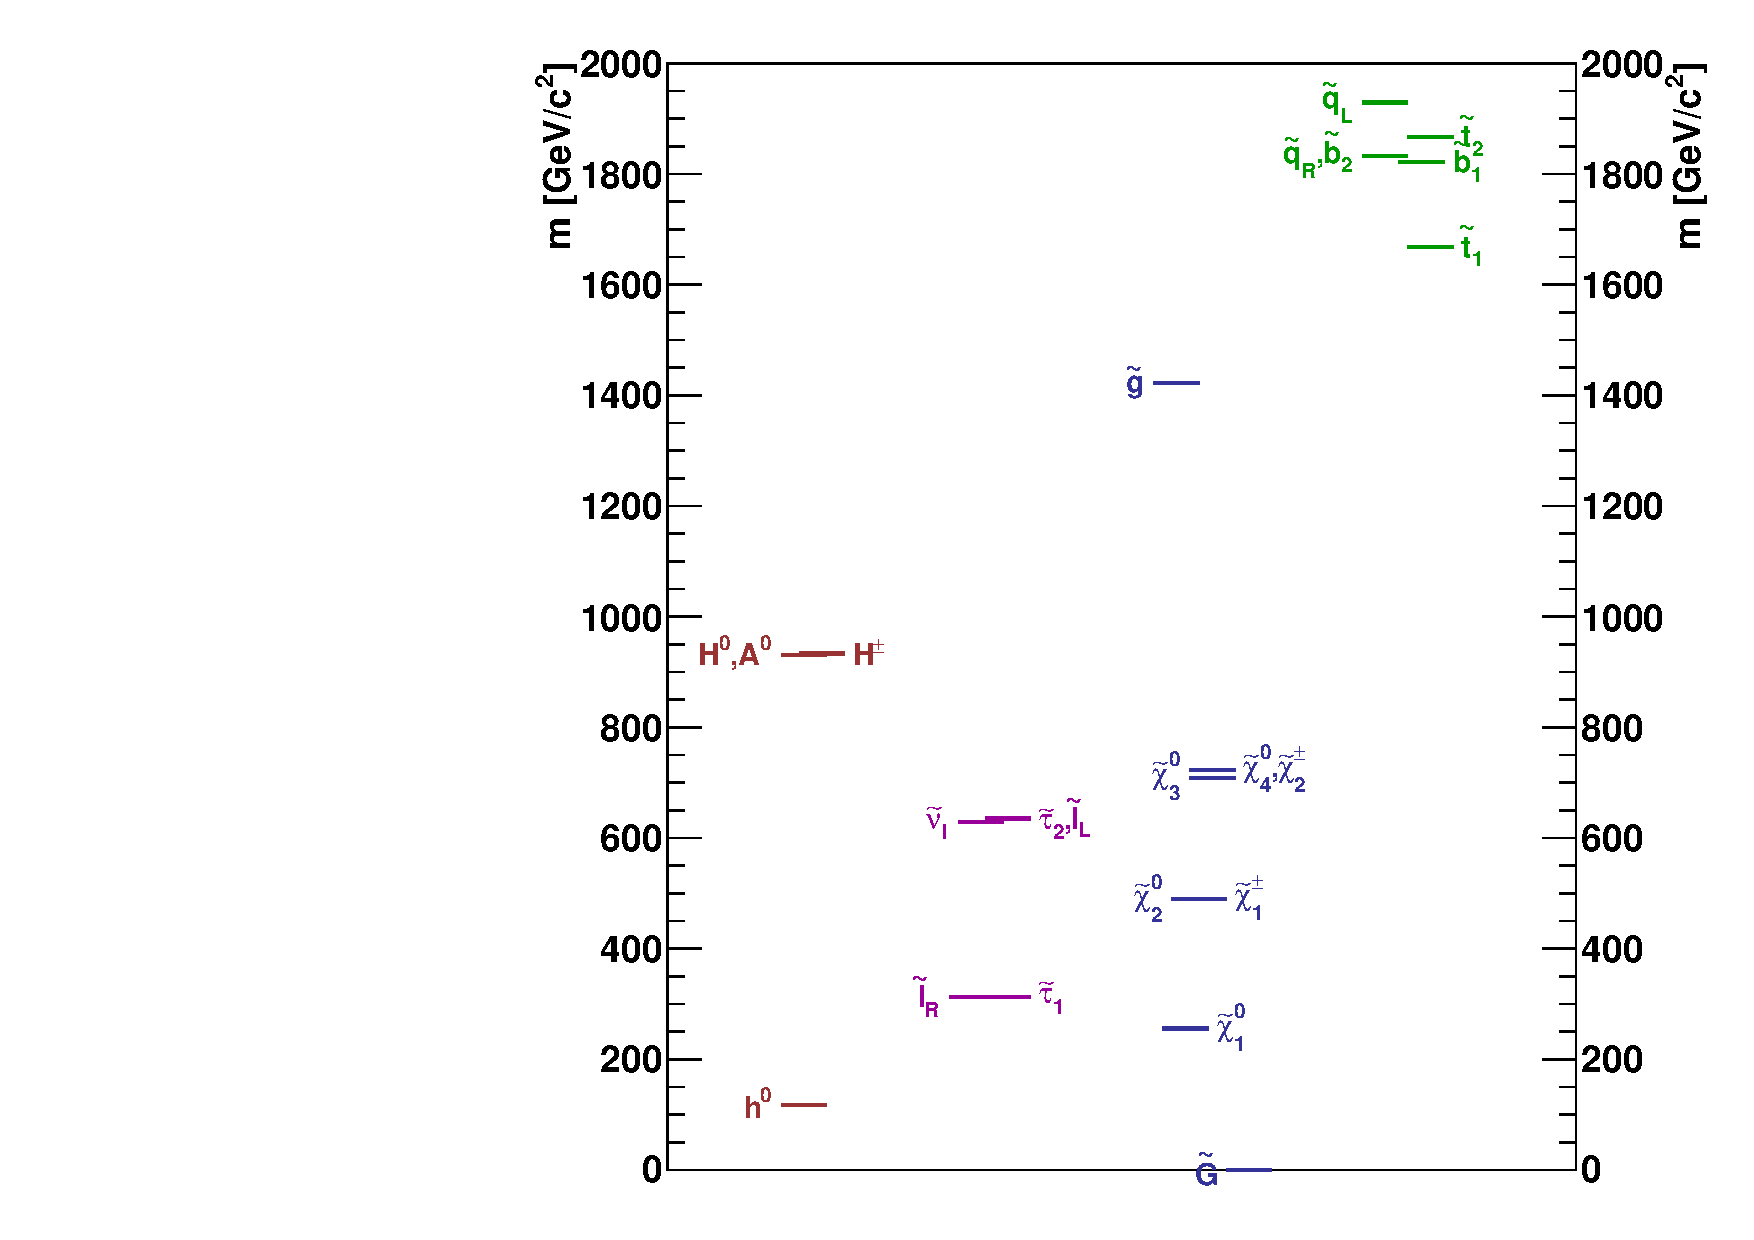
\includegraphics[height=6.0cm,width=0.85\linewidth]{THESISPLOTS/gmsb_Lambda180_CTau10000.pdf}
\end{frame}


%% SUSY at LHC
\begin{frame}
\frametitle{\Huge{Supersymmetry Production}}
 % \begin{tikzpicture}[remember picture,overlay]
 %     \node[at=(current page.center)] {
 %     \includegraphics[width=\paperwidth]{THESISPLOTS/SUSY-XSEC.pdf}
 %           };
 %  \end{tikzpicture}
% \usebackgroundtemplate{\includegraphics[width=\paperwidth]{THESISPLOTS/SUSY-XSEC.pdf}}
 \begin{minipage}[t]{\paperwidth}
   \includegraphics[height=7cm,width=0.80\linewidth]{THESISPLOTS/SUSY-XSEC.pdf}
   
 %\caption{mGMSB:SPS8 model}
 \end{minipage}
 \begin{minipage}[b]{\linewidth}
   SUSY production mostly in strong interactions at LHC.
 \end{minipage}
\end{frame}

%Production & Decay
\begin{frame}
\frametitle{\Huge{Production and Decay }}
 %\begin{columns}
 % \begin{column}{1.\textwidth}
   \begin{minipage}[t]{0.7\linewidth}
 %    \centering
      \includegraphics[width=0.80\paperwidth]{THESISPLOTS/SUSY-DECAY.pdf}
 \end{minipage}
 %\begin{minipage}[b]{0.7\linewidth}
 %\newline \textcolor{blue} {\texttt{Y. Kats et al: arXiv:1110.6444v2}}
 %\end{minipage}
    
\end{frame}    
\begin{frame}
\frametitle{\Huge{Delayed Photon Production}}  
  %  \hspace{5cm}
   % \begin{minipage}[t]{0.5\paperwidth}
 %     \centering 
  \fboxsep=0pt  
  \begin{varblock}[7cm]{Double Photon}
  % \fbox{%
   \centering
    %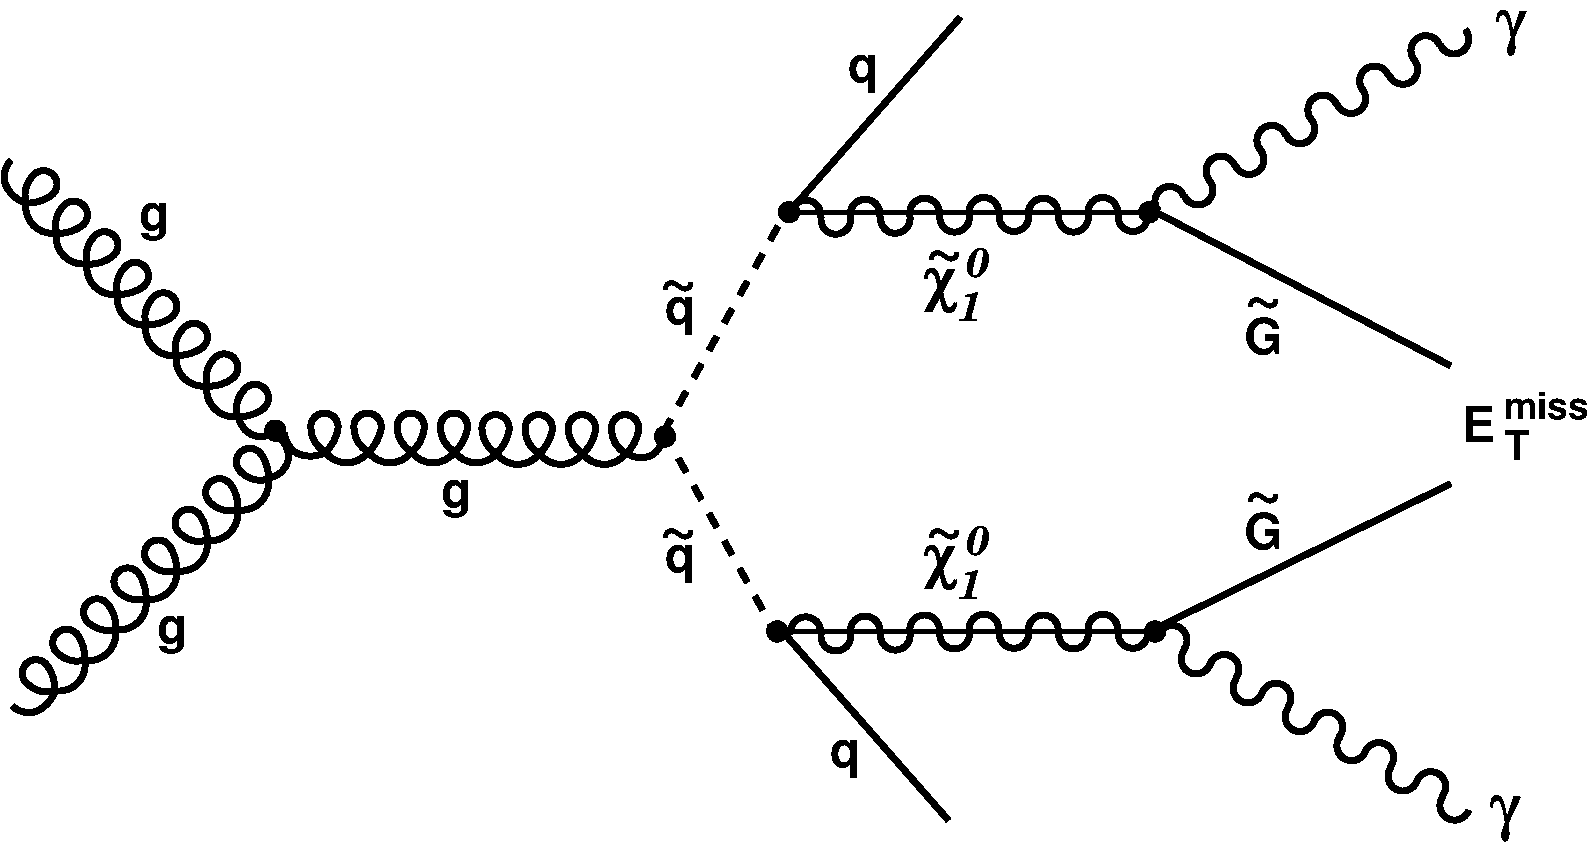
\includegraphics[width=0.50\linewidth]{THESISPLOTS/Diphoton_squark.pdf}
    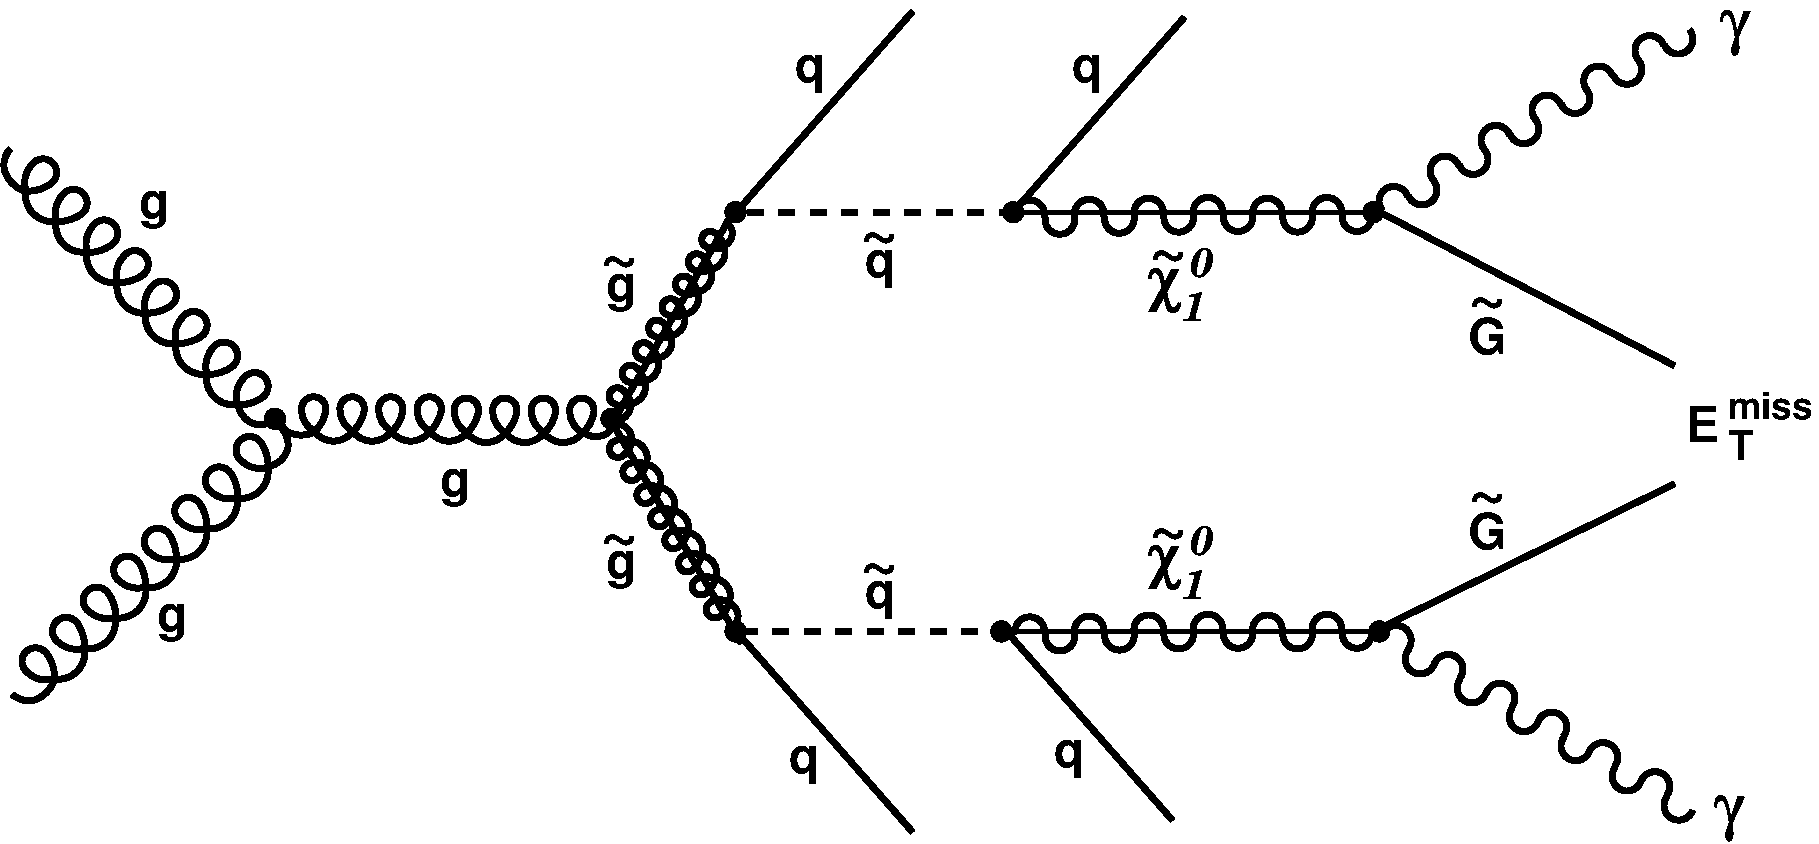
\includegraphics[width=0.50\linewidth]{THESISPLOTS/Diphoton_gluino.pdf}
       
     \large{ \textcolor{red}{2 Photons}, \textcolor{green}{Jets}, \textcolor{blue}{Large MET} }   
   %  }
     \end{varblock}%
     \vspace{-0.3cm}
     \begin{varblock}[7cm]{Single Photon}
  %\fbox{
    \centering
       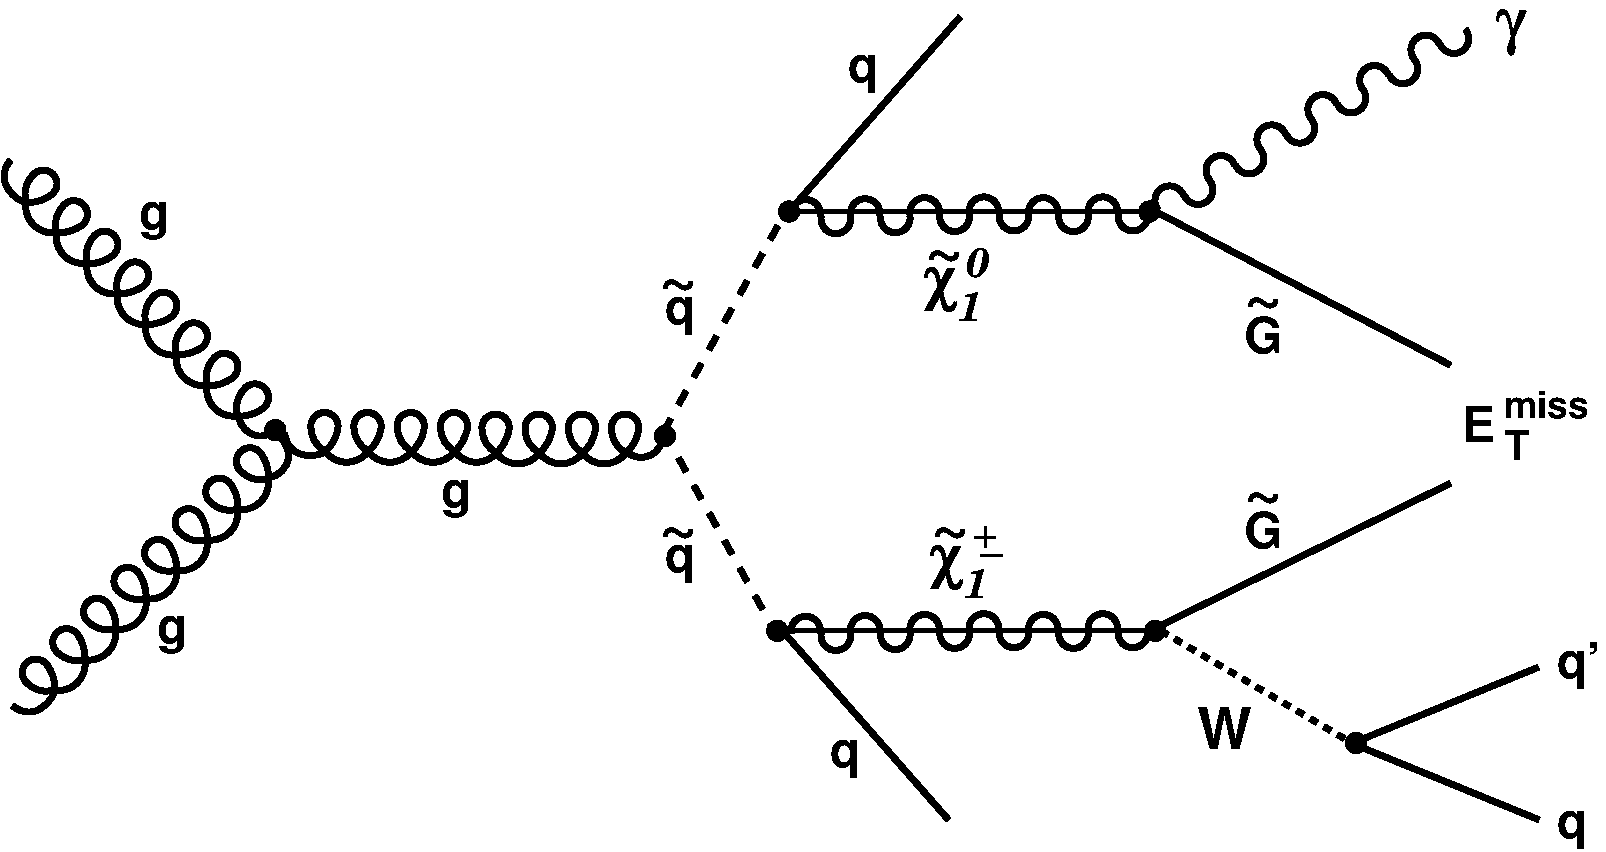
\includegraphics[width=0.50\linewidth]{THESISPLOTS/SinglePhoton_squark.pdf}
       \newline
       \large{ \textcolor{red}{1 Photon}, \textcolor{green}{Jets}, \textcolor{blue}{Large MET} }
  %     }
    \end{varblock}
   % \end{minipage}
 % \end{column}
 % \hspace{-4.5cm}
  % Column 2 begins
%  \begin{column}{0.9\textwidth}  
%    \begin{minipage}[t]{0.5\textwidth}
%     \centering
%      \includegraphics[height=7cm,width=1.1\linewidth]{THESISPLOTS/SUSY-XSEC.pdf}
      %\includegraphics[scale=0.4]{THESISPLOTS/SUSY-XSEC.pdf}
%    \end{minipage}
%    \end{column} 
% \end{columns}     
\end{frame}

% Tranverse Decay Distance
\begin{frame}
\frametitle{\Huge{Tranverse Decay Distance}}
\vspace{-0.70cm}
\begin{minipage}[t]{0.4\paperwidth}
   \begin{varblock}[6cm]{Distance Travelled}
     \begin{displaymath}
       \mathrm{L}_{T} = c\tau\cdot \left(\gamma \beta_{T} \right)  = c\tau \cdot \left(\frac{p_{T}}{m} \right)
      \end{displaymath}
    \end{varblock}
  
   \begin{varblock}[6cm]{Proper Decay Length}
    \begin{displaymath}
    c\tau_{\texttt{NLSP}} = C^{2}_{\texttt{grav}}\frac{1}{\kappa}\left(\frac{m_{\texttt{NLSP}}}{ GeV}\right)^{-5}\left(\frac{\sqrt{\texttt{F}}}{TeV}\right)^{4}
     \end{displaymath}
    \end{varblock}    
\end{minipage} 
  
\begin{minipage}[b]{0.65\paperwidth}
    \includegraphics[width=0.75\paperwidth]{THESISPLOTS/DECAY-RATES.pdf}
     \newline \texttt{\textcolor{blue}{J. Ruderman, D. Shih arXiv:1103.6083}}
\end{minipage} 
   
 % begin{minipage}[b]{0.5\textwidth}
  %\texttt{Y. Kats et al}: arXiv:1110.6444v2
 %\end{minipage}
\end{frame}

%%% Left Column
      %\vspace{-1cm}
      %\fboxsep=0pt  
       %\fbox{%
      % \begin{itemize}
       % \item{ \color{UMN@Maroon} \textbf{ECAL Timing}}

%%% Previous Experiments
\begin{frame}
\frametitle{\Huge{Experiments:ATLAS}}
\begin{minipage}[t]{\paperwidth}
 \begin{tcolorbox}[colback=UNL@Cream!5,colframe=UNL@Cream!40,title=\textcolor{UMN@Maroon}{\textbf{ATLAS}}]
  %\setbeamertemplate{itemize items}{$\mathbb{\rhd*}$} %\otimes, \ominus \dagger etc
 %\begin{itemize}
  %\item \textcolor{UMN@Maroon}{\textbf{ATLAS}}
  %\begin{varblock}[7cm]{\textbf{ATLAS}}
  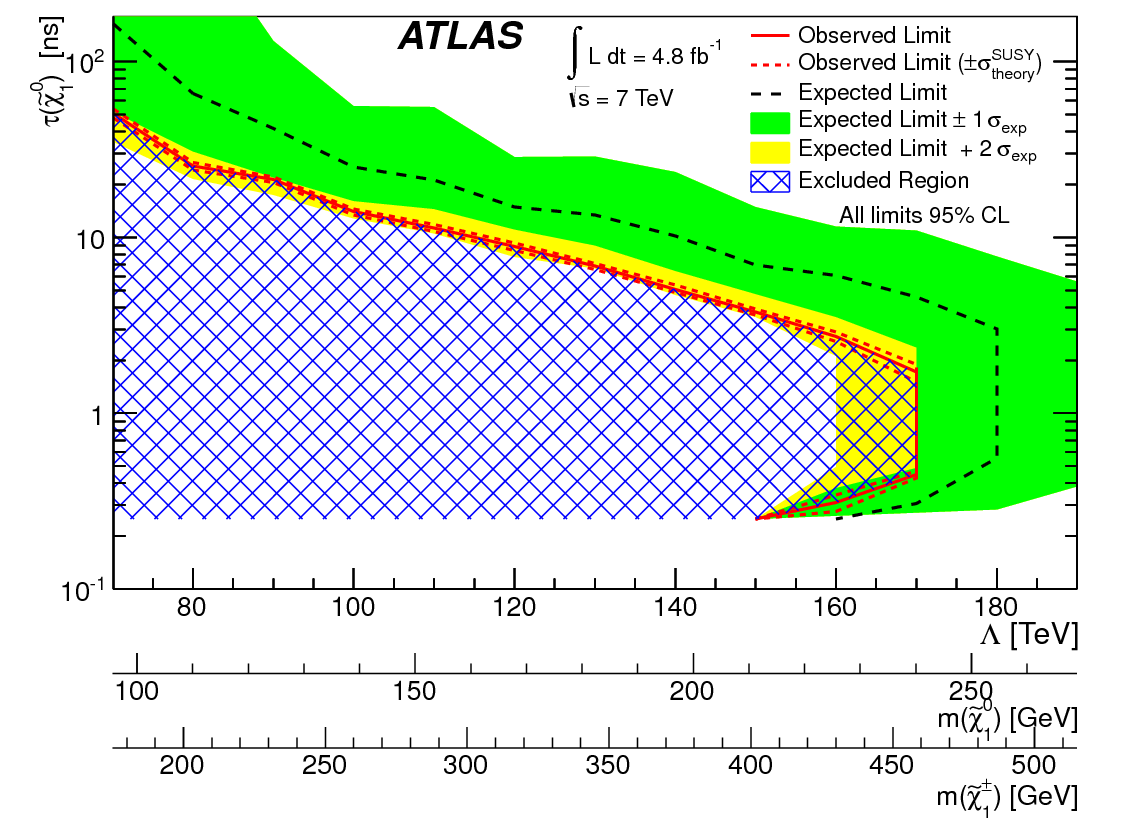
\includegraphics[height=0.50\textwidth,width=0.90\linewidth]{THESISPLOTS/ATLAS_Upper_Limit.png}
  %\end{varblock}
  \end{tcolorbox}
 %\end{itemize}
 
 Excluded: Mass $>  $ and $c\tau >  $.
\end{minipage}
\end{frame}

\begin{frame}
\frametitle{\Huge{Experiments:DO,CDF,CMS }}

\begin{minipage}[b]{\paperwidth}
\begin{tcolorbox}[colback=UNL@Cream!5,colframe=UNL@Cream!40,title=\textcolor{UMN@Maroon}{\textbf{CMS, CDF, DO}}]
 %\setbeamertemplate{itemize items}{$\mathbb{\rhd*}$} %\otimes, \ominus \dagger etc
%\begin{itemize}
%\item \textcolor{UMN@Maroon}{\textbf{DO, CDF, CMS}}
%\begin{varblock}[7cm]{\textbf{CMS, CDF, DO}}
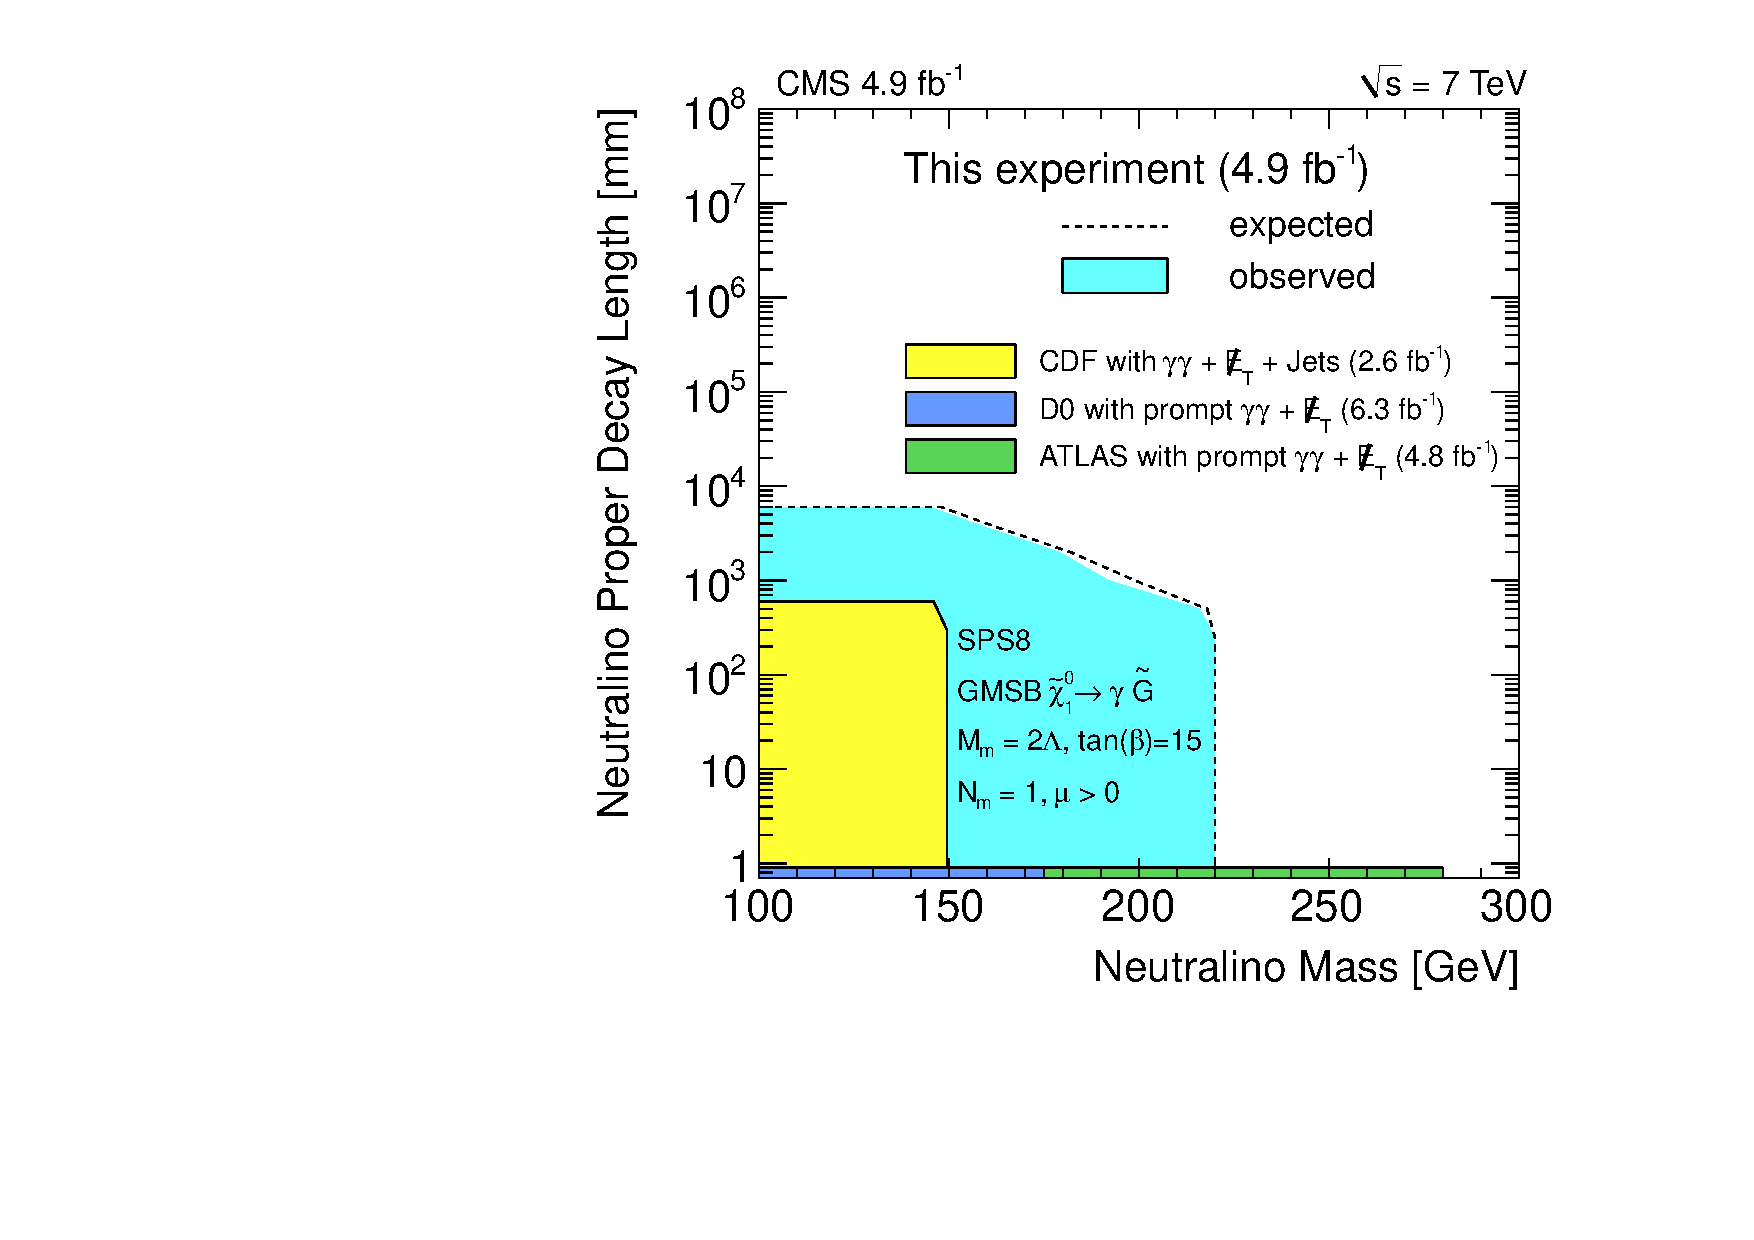
\includegraphics[height=0.55\textwidth,width=0.95\linewidth]{THESISPLOTS/2D_exclusion.pdf}
 \end{tcolorbox}
 %\end{varblock}
 % \end{itemize}
 Excluded: Mass $>  $ and $c\tau >  $.
\end{minipage}
\end{frame}




% ECAL Timing
\section{ECAL TIMING}
{
\usebackgroundtemplate{%
\tikz\node[opacity=0.35] {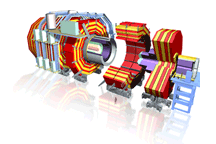
\includegraphics[height=\paperheight,width=\paperwidth]{/home/tensr/Documents/TEN-HEP-PHD-THESIS/PHD_THESIS/PHD/PLOTS/CMS_DET.png}};}
\begin{frame}
   \begin{center}
    \textcolor{UMN@Maroon}{\huge{\textbf{ECAL TIMING}}}
   \end{center}
\end{frame}
}

%% LHC & CMS Detector
\begin{frame}
 \frametitle{\Huge{LHC and CMS}}
 \begin{minipage}[t]{0.85\paperwidth}
  \begin{columns}
   \begin{column}{0.50\linewidth}
 \begin{tcolorbox}[colback=UNL@Cream!5,colframe=UNL@Cream!60,title=\textcolor{UMN@Maroon}{\textbf{\Large{LHC}}}]
    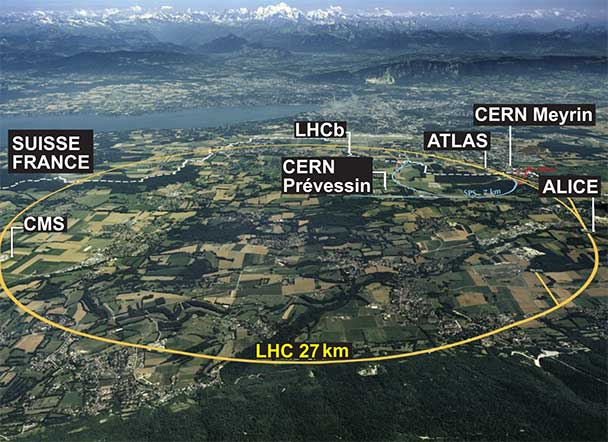
\includegraphics[height=7cm,width=0.99\textwidth]{THESISPLOTS/lhc-ring-aerial_2.jpg}
    \end{tcolorbox}
   \end{column}
   \begin{column}{0.50\linewidth}
   \begin{tcolorbox}[colback=UNL@Cream!5,colframe=UNL@Cream!60,title=\textcolor{UMN@Maroon}{\textbf{
   \Large{CMS Detector}}}]
    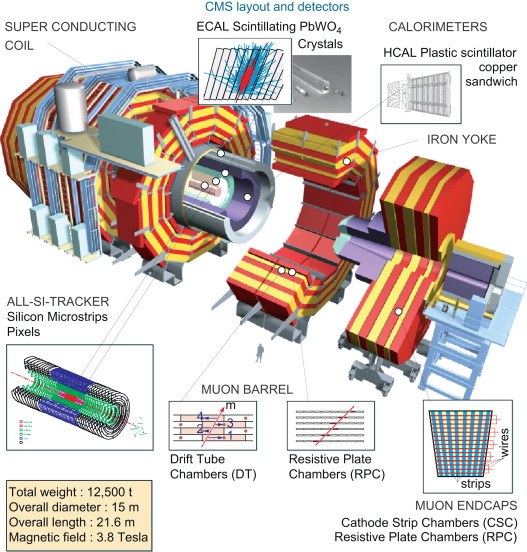
\includegraphics[height=7cm,width=0.99\textwidth]{THESISPLOTS/CMS_LAYOUT_AND_DETECTORS.jpg}
  \end{tcolorbox}
  \end{column}
 \end{columns}
 \end{minipage}
\end{frame}


%ECAL
\begin{frame}
 \frametitle{\Huge{Electromagnetic Calorimeter}}
 % \begin{minipage}[t]{0.70\paperwidth}
 %  \begin{columns}
  %  \begin{column}{0.55\linewidth}
    \begin{tcolorbox}[colback=UNL@Cream!5,colframe=UNL@Cream!70,title=\textcolor{UMN@Maroon}{\textbf{\Large{ECAL Subdetector}}}]
    \mbox{    
    \includegraphics[height=0.25\textwidth,width=0.35\linewidth]{THESISPLOTS/CMS-ECAL-EB-EE.png} \quad
    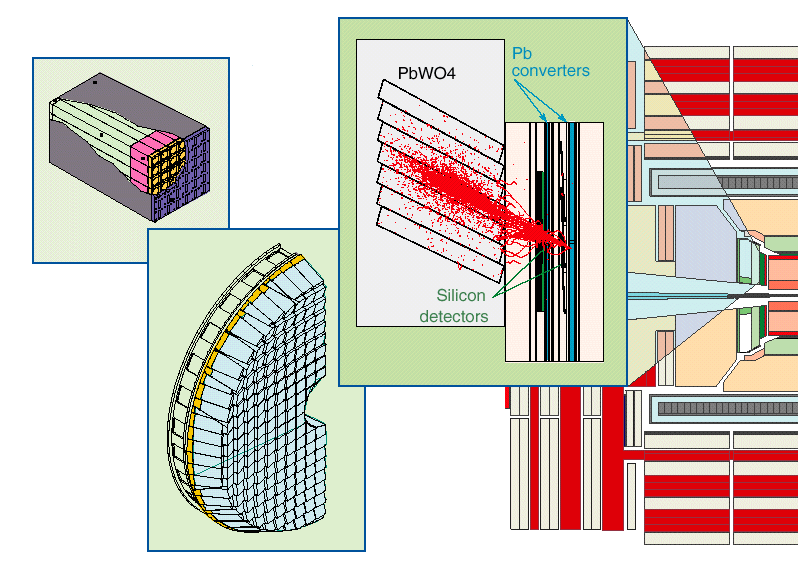
\includegraphics[height=0.25\textwidth,width=0.30\linewidth]{THESISPLOTS/New-Physics-PLOTS/ECAL_Crystals.png} \quad
    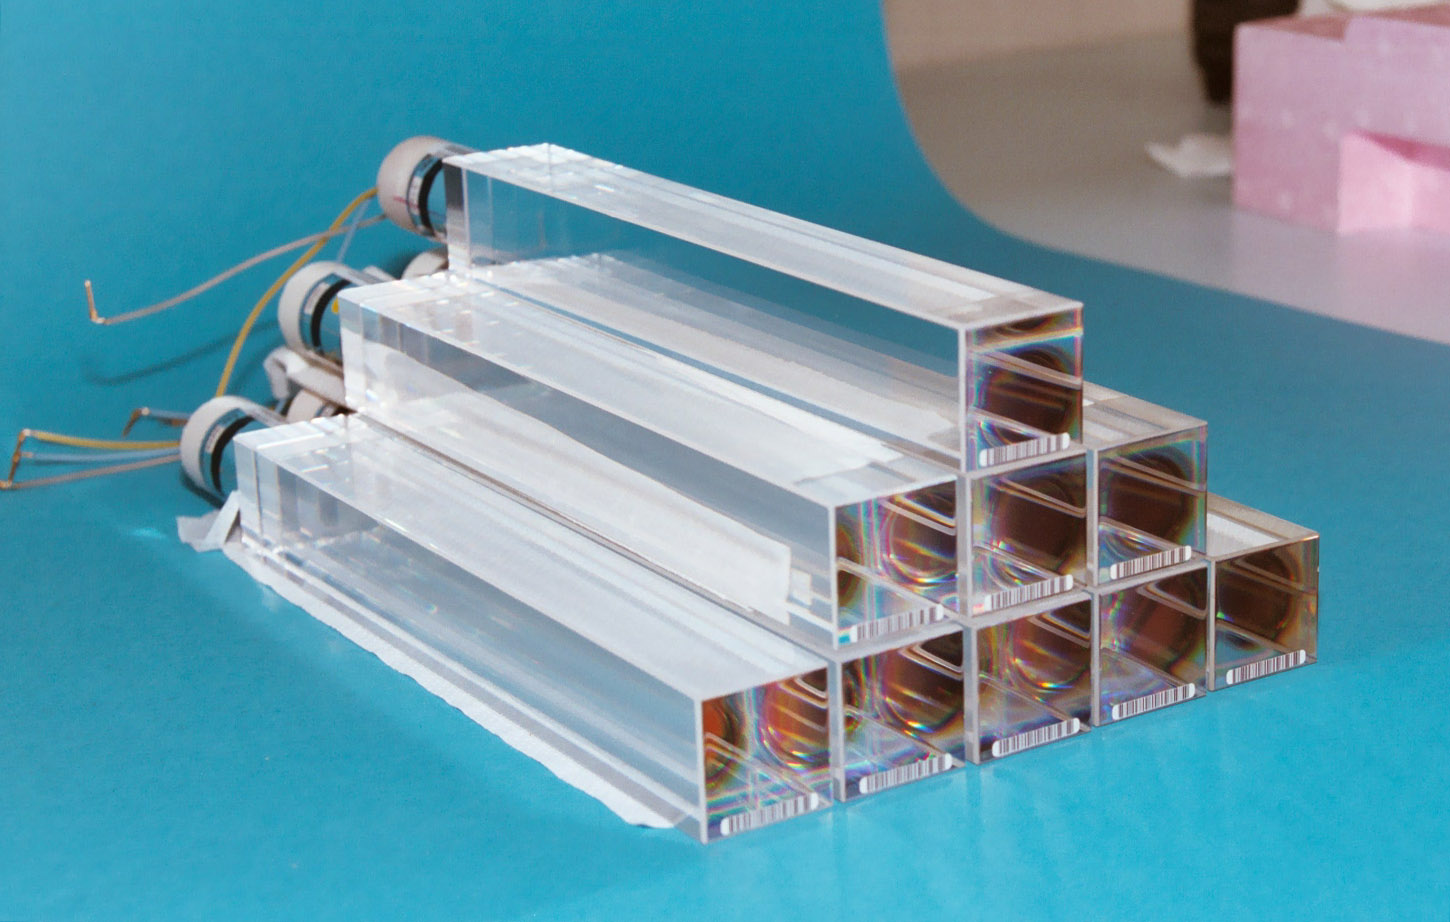
\includegraphics[height=0.25\textwidth,width=0.30\linewidth]{THESISPLOTS/New-Physics-PLOTS/CMS-ECAL-CRYS.jpg}
    }
 \textbf{Barrel Detector~(EB)}:  $|\eta| < 1.475$. \quad \\
  \textbf{Endcap Detectors~(EE)}: $1.5 < \eta < 3.0$..
  
    \end{tcolorbox} 
%    \end{column}
%    \begin{column}{0.55\linewidth}
%    \begin{tcolorbox}[colback=UNL@Cream!5,colframe=UNL@Cream!70,title=\textcolor{UMN@Maroon}{\textbf{Endcap Detectors.}}]
 %    \includegraphics[height=0.35\textwidth,width=0.65\linewidth]{/THESISPLOTS/CMS-ECAL-EB-EE.png}
   
 %   \end{tcolorbox}
 %    \end{column}
%   \end{columns}   
%   \end{minipage}
   \vspace{-0.1cm}
%   \begin{minipage}[b]{0.82\paperwidth}
    \begin{columns}
    \begin{column}{0.73\linewidth}
      \begin{tcolorbox}[colback=UNL@Cream!5,colframe=UNL@Cream!70,title=\textcolor{UMN@Maroon}{\textbf{\large{ECAL Properties}}}]
         \setbeamertemplate{itemize items}{$\mathbb{\triangleright}$} %\otimes, \ominus \dagger etc   
      \begin{itemize}
       \normalsize{
        \item 75,848 Lead Tungstate crystals,
        \item Crystals measure energy and time,
        \item Shower in crystal generates lights detected using:
         \setbeamertemplate{itemize items}{$\mathbb{\star}$}
          \begin{itemize}
           \item \tiny{Avalanche Photo-Diodes(APD) in EB,}
           \item \tiny{Vacuum Photo-Triodes(VPT) in EE}
          \end{itemize}
        \setbeamertemplate{itemize items}{$\mathbb{\triangleright}$} %\otimes, \ominus \dagger etc
        \vspace{-0.30cm} 
        \item Readout with custom ASICs.% in 250~nm CMOS.
       }
      \end{itemize}
    
      \end{tcolorbox} 
     \end{column} 
     \begin{column}{0.38\linewidth}
       \begin{tcolorbox}[colback=UNL@Cream!5,colframe=UNL@Cream!70,title=\textcolor{UMN@Maroon}{\textbf{\large{Readout Chain}}}]     
        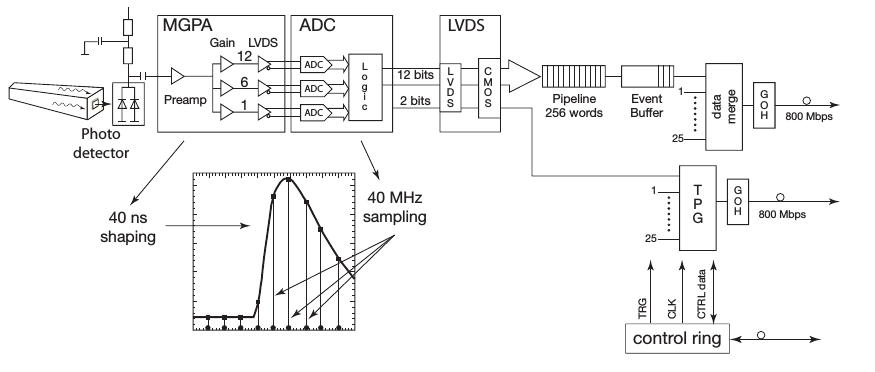
\includegraphics[height=1.0\textwidth,width=0.95\linewidth]{THESISPLOTS/ReadOut.png}     
       \end{tcolorbox} 
     \end{column}
   \end{columns}
   
% \end{minipage}    
 
\end{frame}






% ECAL Timing
\begin{frame}
\frametitle{\Huge{ECAL Time Measurement}}
 \begin{minipage}[t]{\paperwidth}
       \begin{tcolorbox}[colback=UNL@Cream!5,colframe=UNL@Cream!70,title=\textcolor{UMN@Maroon}{\textbf{\Large{Time Reconstruction}}}]
   %\item\textcolor{UMN@Maroon}{\textbf{Time Reconstruction}} 
   \begin{columns}
  %\begin{itemize} 
    \begin{column}{0.450\linewidth}
    \setbeamertemplate{itemize items}{$\mathbb{\rhd*}$} %\otimes, \ominus \dagger etc
         \begin{itemize}
          \item 10 digitized samples.
          \item Extract time using Fit or Weighted algorithm.
         \end{itemize}      
    \end{column}
    \begin{column}{0.75\linewidth}
    \mbox{
         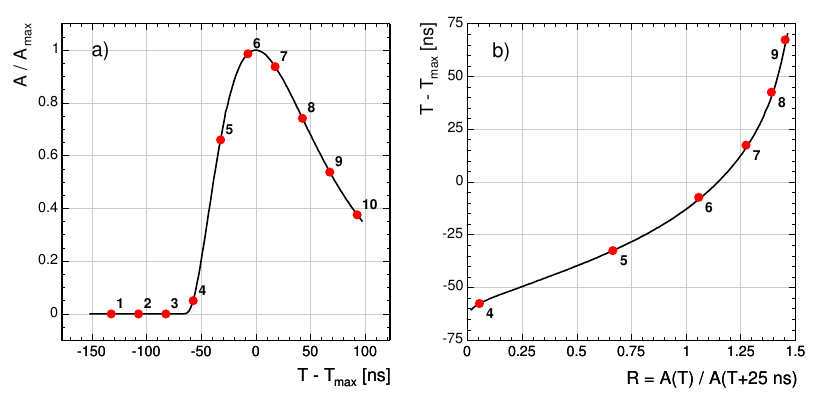
\includegraphics[height=0.30\textwidth, width=0.65\linewidth]{THESISPLOTS/AmplitudeVsTMax.png} 
         %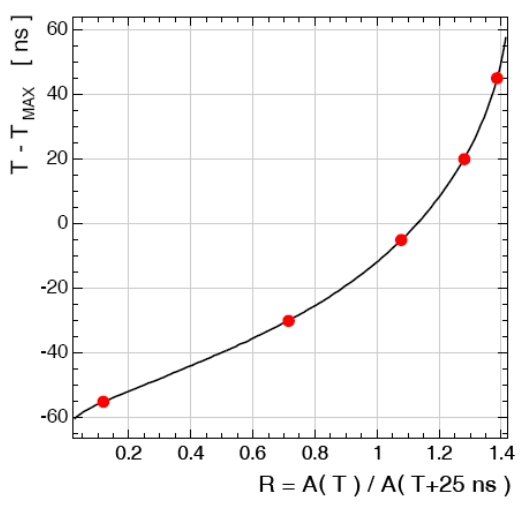
\includegraphics[height=0.58\textwidth, width=0.55\linewidth]{THESISPLOTS/TMaxPhaseVsRatio.png}
         }
     %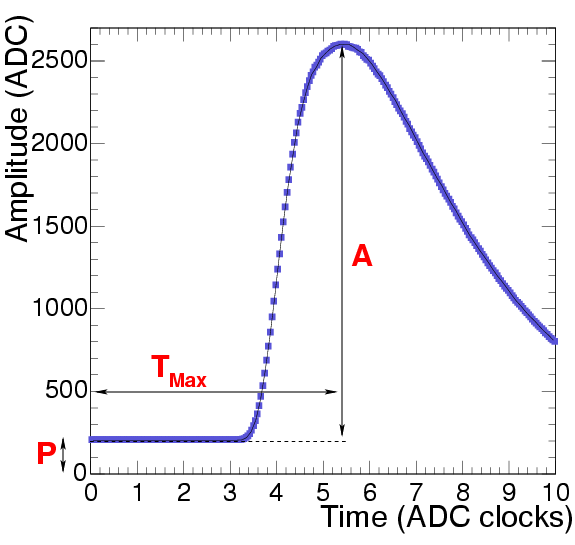
\includegraphics[height=0.40\textwidth,width=0.90\linewidth]{THESISPLOTS/Time_Amplitude_Profile.png}
    \end{column} 
     %\end{itemize} 
   \end{columns}  
 \end{tcolorbox}
 
%\end{minipage}
%\vspace{-0.1cm} 
%\begin{minipage}[b]{0.95\paperwidth}
    \begin{tcolorbox}[colback=UNL@Cream!5,colframe=UNL@Cream!70,title=\textcolor{UMN@Maroon}{\textbf{Time Measurement}}]    
   %\item \textcolor{UMN@Maroon}{\textbf{Time Measurement}}
      %\begin{equation*}\label{eq:avetime}
     %\end{equation}
    %\item{ \color{UMN@Maroon} \textbf{ECAL Time Resolution}}    
  \begin{columns}
    \begin{column}{0.37\textwidth} 
     %%% Left Column
      %\vspace{-1cm}
      %\fboxsep=0pt  
       %\fbox{%
       \setbeamertemplate{itemize items}{$\mathbb{\rhd*}$} %\otimes, \ominus \dagger etc
      \begin{itemize}
       \item{ \color{UMN@Maroon} \textbf{Error Weighted}}\\ 
       \end{itemize}
       %\textcolor{UMN@Maroon}{\textbf{Error Weighted:}}
       %\begin{equation*}
        $ T_{MAX} = \frac{{\displaystyle\sum_{i}} \frac{T_{MAX,i} }{\sigma_i^2} }{ {\displaystyle\sum_{i}} \frac{1}{\sigma_i^2} } $ \\
      % \end{equation*}
        \end{column}
     \end{columns}      
        
       % \begin{column}{0.36\textwidth}
         %\setbeamertemplate{itemize items}{$\mathbb{\rhd\bullet}$} %\otimes, \ominus \dagger etc
        % \begin{itemize}     
        %   \item{
        %    \color{UMN@Maroon} \textbf{Fit Method}}
        %\end{itemize}
        %\textcolor{UMN@Maroon}{\textbf{Fit Method:}}
         
        %\end{column}%          
           %\begin{itemize}
           %  \item ECAL timing resolution $\sigma_{t} < 500$~ps.
            % \item Use timing to identify photons and electrons from long-lived decay.
           %\end{itemize}
       % \end{itemize}              
    
% Right Column
     % \hspace{0.5cm}
     %\begin{column}{0.60\textwidth}
           
    % \end{column} 
   
     
  %\end{itemize}
  \end{tcolorbox}
\end{minipage}
\end{frame}

\begin{frame}
\frametitle{\Huge{ECAL Time Resolution}}
Time Resolution Equation and parameter Definitions.

\end{frame}

   
\begin{frame}
\frametitle{\Huge{Test Beam Performance}}
 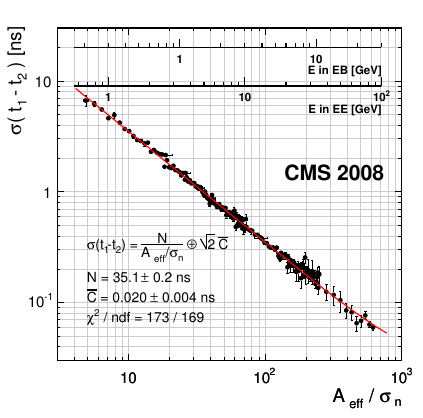
\includegraphics[height=0.65\paperwidth,width=0.85\paperwidth]{THESISPLOTS/ECAL_Timing_Resolution.png}   
\end{frame}   
   
 % Timing Calibration
\begin{frame}
\frametitle{Timing Calibration}
\begin{minipage}[b]{0.85\paperwidth}
 \begin{tcolorbox}[colback=UNL@Cream!5,colframe=UNL@Cream!70,title=\textcolor{UMN@Maroon}{\textbf{Calibration Procedure}}] 
  \begin{columns}
   \begin{column}{0.55\linewidth}
   \setbeamertemplate{itemize items}{$\mathbb{\rhd*}$} %\otimes, \ominus \dagger etc
    \begin{itemize}
      \item Adjust Crystal time such that $ \left\langle t^{\gamma}_{crys} \right\rangle \approx 0$
      \item Average is over events(\textit{rechits})/crystal.
    \end{itemize}
    \end{column}
    \begin{column}{0.65\linewidth}
     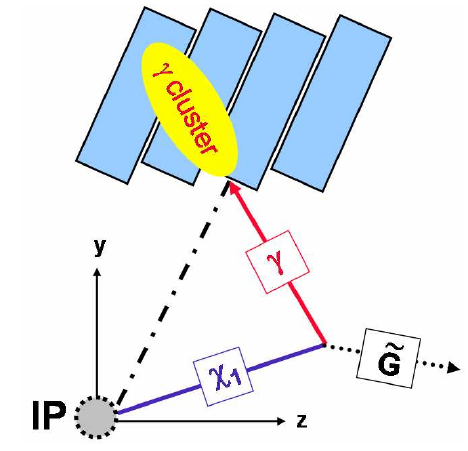
\includegraphics[height=0.35\textwidth, width=0.63\linewidth]{THESISPLOTS/TimeCalibIdea.png}
     
     \end{column}
    \end{columns}      
  \end{tcolorbox}
\end{minipage}
\begin{minipage}[b]{0.83\paperwidth}
 \begin{columns}
   \begin{column}{0.50\linewidth}
     \begin{tcolorbox}[colback=UNL@Cream!5,colframe=UNL@Cream!70,title=\textcolor{UMN@Maroon}{\textbf{Before Calibration}}] 
       \mbox{
            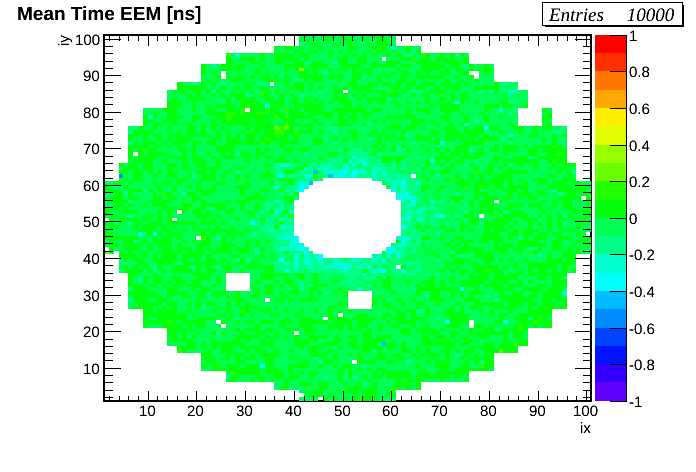
\includegraphics[height=0.45\textwidth, width=0.53\linewidth]{THESISPLOTS/calibDiffMapEEM_Before_CALIB.png} 
            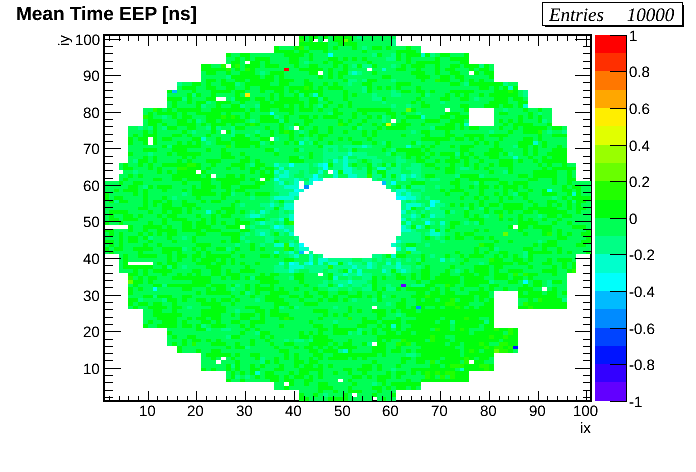
\includegraphics[height=0.45\textwidth, width=0.53\linewidth]{THESISPLOTS/calibDiffMapEEP_Before_CALIB.png} }
            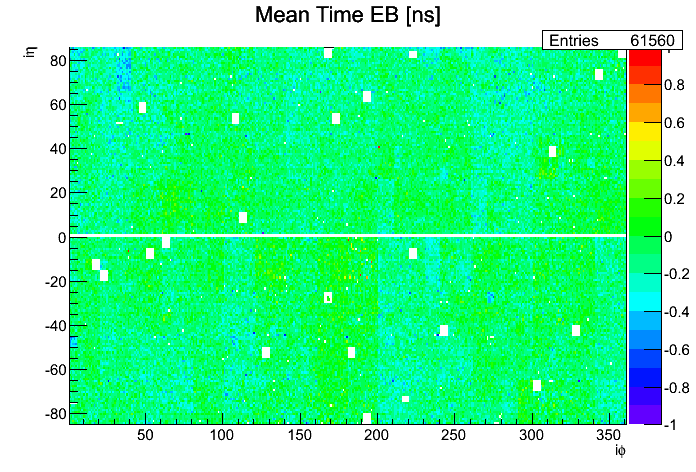
\includegraphics[height=0.45\textwidth, width=0.93\linewidth]{THESISPLOTS/calibDiffMapEB_Before_Calibration.png}
     \end{tcolorbox}
     \end{column}
     \begin{column}{0.50\linewidth}
       \begin{tcolorbox}[colback=UNL@Cream!5,colframe=UNL@Cream!70,title=\textcolor{UMN@Maroon}{\textbf{After Calibration}}] 
      \mbox{            
            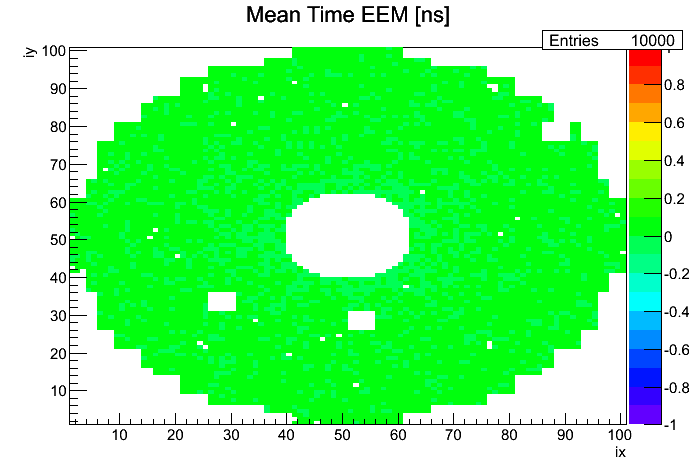
\includegraphics[height=0.45\textwidth, width=0.53\linewidth]{THESISPLOTS/calibDiffMapEEM_AFter_CALIB.png}
            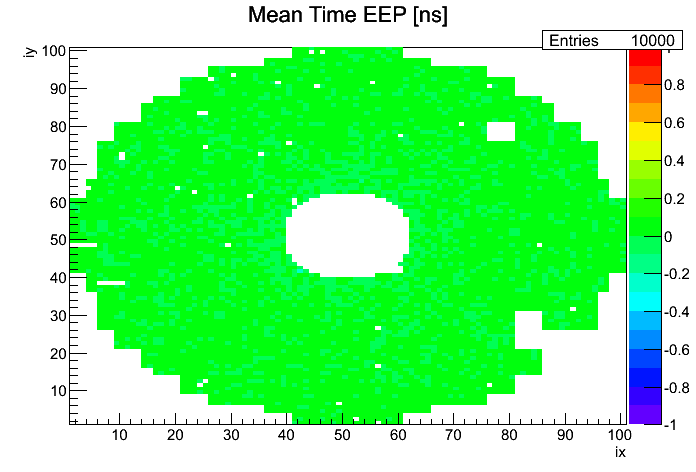
\includegraphics[height=0.45\textwidth, width=0.53\linewidth]{THESISPLOTS/calibDiffMapEEP_After_CALIB.png} }
            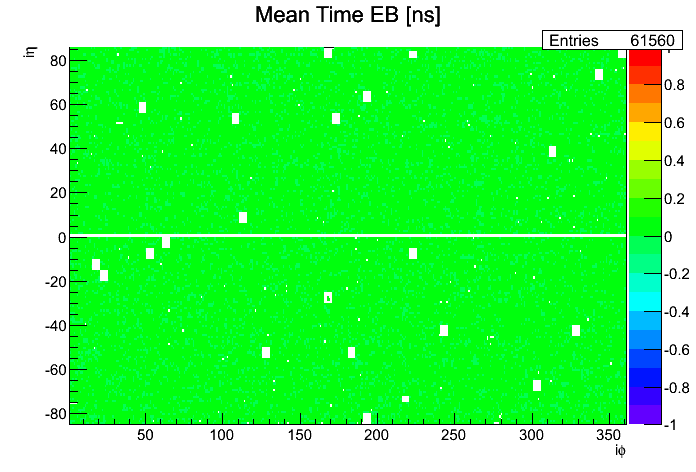
\includegraphics[height=0.45\textwidth, width=0.93\linewidth]{THESISPLOTS/calibDiffMapEB_After_Calibration.png}
      
     \end{tcolorbox}     
    \end{column}
   \end{columns} 
 \end{minipage}
\end{frame}
   
   
  
   
 % Timing Performance  
\begin{frame}
\frametitle{ECAL Timing Performance}
\begin{minipage}[b]{0.85\paperwidth}
  %\begin{itemize}
    %\item \textcolor{UMN@Maroon}{\textbf{Timing Resolution}}
  \begin{tcolorbox}[colback=UNL@Cream!5,colframe=UNL@LightGrey!70,title=\textcolor{UMN@Maroon}{\textbf{ECAL Timing Resolution}}]
  \setbeamertemplate{itemize items}{$\mathbb{\rhd\dag}$} %\otimes, \ominus \dagger etc
     \begin{itemize}
     \item  Time resolution better than $150$~ps for $E > 50$ ~GeV
     \end{itemize}
  \begin{columns}
   \begin{column}{0.50\linewidth}
     \begin{tcolorbox}[colback=UNL@Cream!5,colframe=UNL@Cream!70,title=\textcolor{UMN@Maroon}{\textbf{Test Beam }}] 
    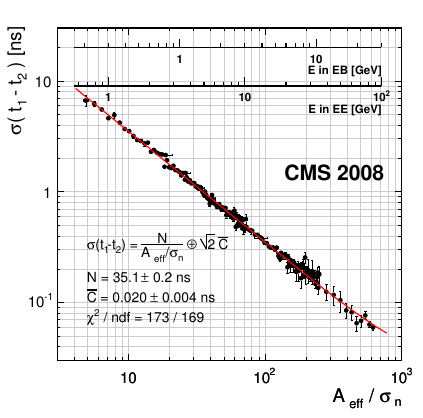
\includegraphics[height=5.0cm,width=\textwidth]            {THESISPLOTS/ECAL_Timing_Resolution.png}
    \end{tcolorbox}
   \end{column}
   \begin{column}{0.55\linewidth}
     \begin{tcolorbox}[colback=UNL@Cream!5,colframe=UNL@Cream!70,title=\textcolor{UMN@Maroon}{\textbf{LHC RUN I}}]
      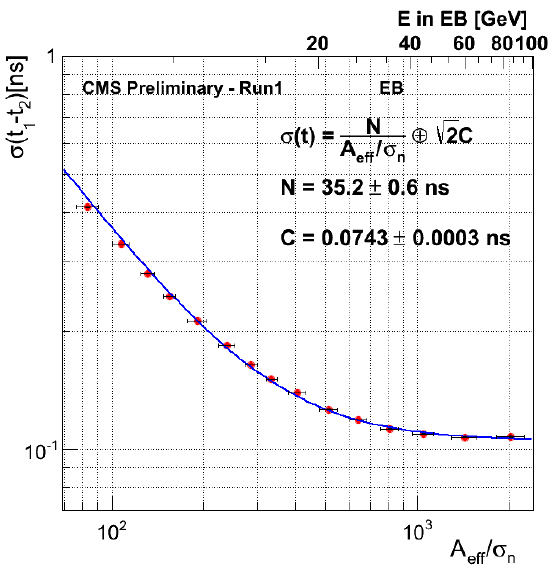
\includegraphics[height=5.0cm,width=\textwidth]            {THESISPLOTS/NeigboMethodECALTimeRes.png}
     \end{tcolorbox} 
     \end{column} 
    \end{columns} 
   \end{tcolorbox}
  \end{minipage}   
\end{frame}

%continuation of Timing
\begin{frame}
\frametitle{ECAL Photon Arrival Time}
  \begin{minipage}[t]{0.83\paperwidth} 
    \setbeamertemplate{itemize items}{$\mathbb{\rhd*}$} %\otimes, \ominus \dagger etc
        \begin{enumerate}
         \item $T_{\gamma} =$ Error weighted average time of crystals in photon.
         \item $T_{\gamma} =$ Seed (most energetic) crystal time.        
        \end{enumerate}
        \begin{tcolorbox}[colback=UNL@Cream!5,colframe=UNL@Cream!70,title=\textcolor{UMN@Maroon}{\textbf{Photon Arrival Time}}] 
      % \item \textcolor{UMN@Maroon}{\textbf{Photon Timing}}
       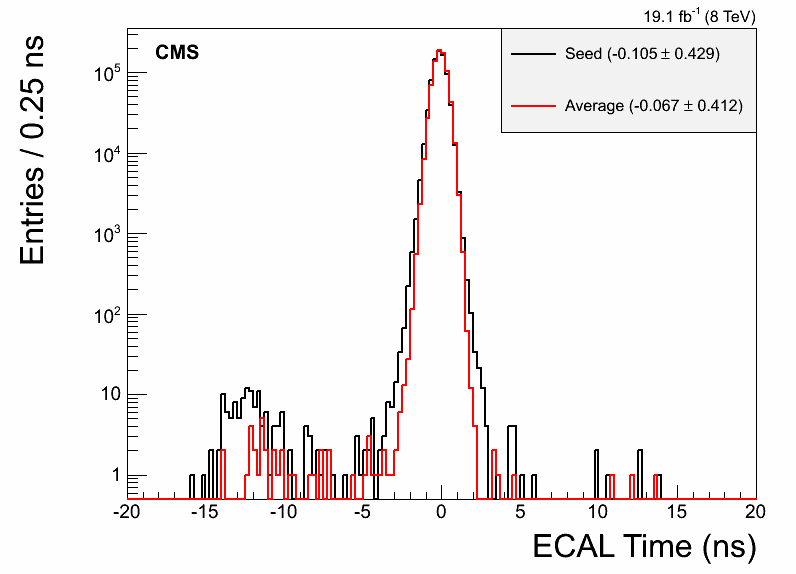
\includegraphics[height=4.5cm,width=0.70\linewidth]                     {THESISPLOTS/AverageVsSeedTime_ECAL.png}   
        \end{tcolorbox}
 \end{minipage}
 \begin{minipage}[b]{\linewidth}
 \setbeamertemplate{itemize items}{$\mathbb{\rhd*}$} %\otimes, \ominus \dagger
        \begin{itemize}
         \item  Similar time in seed and average.
          \item  Photon time = Seed crystal time.
        \end{itemize}
 \end{minipage}
\end{frame}
	
%%% MC Vs Data Time
\begin{frame}
\frametitle{MC Vs Data ECAL Timing}
  \begin{minipage}[t]{0.82\paperwidth}
    \begin{columns}
     \begin{column}{0.50\linewidth}
       \begin{tcolorbox}[colback=UNL@Cream!5,colframe=UNL@Cream!70,title=\textcolor{UMN@Maroon}{\textbf{Before Correction }}] 
          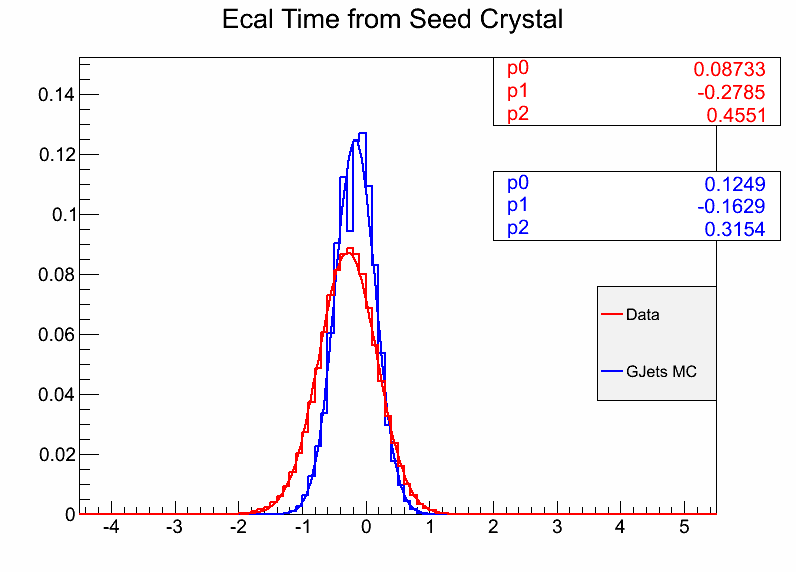
\includegraphics[height=5.0cm,width=\textwidth]            {THESISPLOTS/SeedTime_data-mc.png}
       \end{tcolorbox}
     \end{column}
     \begin{column}{0.50\linewidth}
       \begin{tcolorbox}[colback=UNL@Cream!5,colframe=UNL@Cream!70,title=\textcolor{UMN@Maroon}{\textbf{After Correction}}] 
             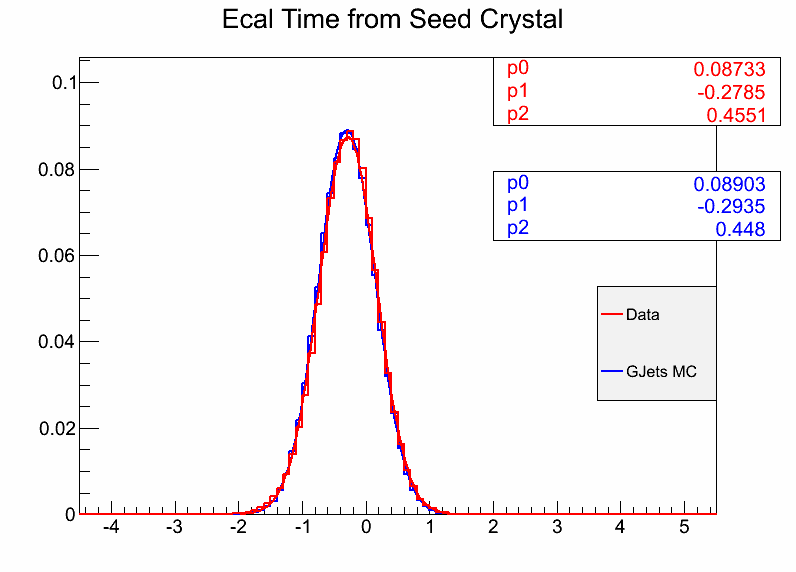
\includegraphics[height=5.0cm,width=\textwidth]            {THESISPLOTS/SeedTime_data-mc_Calib.png}
       \end{tcolorbox}
     \end{column}
  \end{columns}     
\end{minipage}
\begin{minipage}[b]{\linewidth}
  \setbeamertemplate{itemize items}{$\mathbb{\rhd*}$} %\otimes, \ominus \dagger
    \begin{itemize}
     \item Timing corrections from data applied to $\gamma +$ Jets MC.
     \item Data/MC better agreement with corrections applied.
   \end{itemize}
  \end{minipage}
\end{frame}




\section{SEARCH ANALYSIS}
{
\usebackgroundtemplate{%
\tikz\node[opacity=0.35] {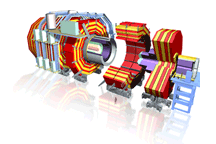
\includegraphics[height=\paperheight,width=\paperwidth]{/home/tensr/Documents/TEN-HEP-PHD-THESIS/PHD_THESIS/PHD/PLOTS/CMS_DET.png}};}
\begin{frame}
   \begin{center}
    \textcolor{UMN@Maroon}{\Huge{\textbf{SEARCH ANALYSIS}} }
   \end{center}
\end{frame}
}

%DataSet and Trigger Section
%\section{Dataset and Trigger}
\begin{frame}
\frametitle{Datasets}
%\hspace{-0.2cm}
\begin{minipage}[b]{0.7\paperwidth}
\begin{itemize}
 \item  \textcolor{UMN@Maroon}{\textbf{Data~($19.1 fb^{-1} $)}}
  %\begin{varblock}[7cm]{Data~($19.1 fb^{-1}$) and Signal MC}
   %\centering
   \tinyv{
   \begin{tabular}{l l p{1.2cm}|p{1.9cm}|}
    \hline
       \bfseries{Dataset Name} & \bfseries{Recorded Luminosity} $ [fb^{-1}]$ \\ %$[\fbinv]$ \\
       \hline
       \texttt{/Run2012B/SinglePhoton/EXODisplacedPhoton-PromptSkim-v3 } & 5.1 \\
       \texttt{/Run2012C/SinglePhoton/EXODisplacedPhoton-PromptSkim-v3 } & 6.9 \\
       \texttt{/Run2012D/SinglePhoton/EXODisplacedPhoton-PromptSkim-v3 } & 7.1 \\
       \hline\hline
       \texttt{/Run2012C/Cosmics/Run2012C-22Jan2013-v1/RECO } & 3130384(\texttt{events}) \\
       \texttt{/Run2012D/Cosmics/Run2012C-22Jan2013-v1/RECO } & 52430 (\texttt{events}) \\
       \hline\hline
       \texttt{/SingleElectron/Run2012A-22Jan2013-v1/AOD} & 5.2 \\
       \texttt{/DoubleElectron/Run2012C-22Jan2013-v1/AOD} & 4.8 \\ 
       \hline \hline     
   \end{tabular}
       }
   \end{itemize}
 \end{minipage}
   % \vspace{1cm}
   % \hspace{0.5cm}
    
 \begin{minipage}[b]{0.7\paperwidth}
 \begin{itemize}
    \item  \textcolor{UMN@Maroon}{\textbf{Signal MC [GMSB~(SPS8)]}}
    %\centering
    \tiny{
    
%     \begin{tabular}{l l l l}
%     %\hline
%       %\textbf{Signal MC [mGMSB~(SPS8)]}
%        \hline
%        \bfseries{$\Lambda$}~[TeV] & \bfseries{$c\tau$}~(mm) & \bfseries{$\sigma_{LO}$}~(pb) & \bfseries{Number of events}\\
%       \hline
%       100 & 250-12,000  & 0.368  & 60,000 \\
%       120 & 250-12,000  & 0.133  & 60,000 \\
%       140 & 250-12,000  & 0.0574 & 60,000 \\
%       160 & 250-12,000  & 0.0277 & 60,000 \\
%       180 & 250-12,000  & 0.0145 & 60,000 \\
%       \hline \hline
%       \end{tabular} 
%\renewcommand\arraystretch{1.2}
%\centering
\begin{tabular}{c c c c c c c}
\hline \hline
$\Lambda$~[TeV] & 100  &   120  &  140  &  160  &  180  &  300  \\
\hline
$M_{\tilde{\chi}^{0}_{1}}$~[$GeV/c^{2}$] & 140 &   169  &  198  &  227  &  256  &  430  \\
\hline
$c\tau$         &  215   &   325  &   130 &   245 &   185 &       \\
 (mm)     &  425   &   645  &   515 &   490 &   365 &   495 \\
                 &  1700  &  1290  &  1030 &   975 &   730 &       \\
                 &  3400  &  1935  &  2060 &  1945 &  1100 &   995 \\
                 &  5100  &  2955  &  2920 &  2930 &  2195 &  2960 \\
                 &  6000  &  3870  &  3985 &  3910 &  3950 &       \\
                 &  9300  &  5985  &  6000 &  5875 &  5980 &  6000 \\
                 &        &  9825  & 10450 &  9815 & 10450 & 10450 \\
\hline \hline
    \end{tabular}
    
}
        
    \end{itemize} 

\end{minipage} 
 
 \begin{minipage}[b]{0.7\paperwidth}
 \begin{itemize}
   \item \textcolor{UMN@Maroon}{ \textbf{$\gamma +$ Jets MC}}
     \mytiny{  
     \begin{tabular}{l l l}
        %\hline
         %
       \hline
        $\hat{p}_{T}$~[GeV\ /c] & $\sigma_{LO}$~(pb) & \bfseries{Number of events}\\
       \hline
       $50 - 80$ & 3322.3  & 1995062 \\
       $80 - 120$ &  558.3  & 1992627 \\
       $120 - 170$  &  108.0 & 2000043 \\
       $170 - 300$  &  30.1 & 2000069 \\
       $300 - 470$  &  2.1  & 2000130 \\
       $470 - 800$  & 0.212 & 1975231 \\
       \hline \hline
       \end{tabular}  
       }
    \end{itemize}
     
    \end{minipage}
% \end{varblock} 
 \end{frame}
 
 % HLT Trigger
 \begin{frame}
 \frametitle{HLT Trigger}
  \begin{minipage}[t]{0.83\paperwidth}
  %\begin{varblock}[7.2cm]{HLT-Trigger Efficiency}
   \begin{tcolorbox}[colback=UNL@Cream!5,colframe=UNL@Cream!70,title=\textcolor{UMN@Maroon}{\textbf{HLT\_DisplacedPhoton65\_CaloIdVL\_IsoL\_PFMET25}}] 
     %\item \textbf{HLT\_DisplacedPhoton65\_CaloIdVL\_IsoL\_PFMET25}%~(\texttt{Main Trigger})
     %\begin{itemize}
     %   \item  HLT\_Photon50\_CaloIdVL\_IsoL (\texttt{Study Trigger})
     %\end{itemize}
   %\end{itemize}  
  %\end{varblock}
 \begin{columns}
    \begin{column}{0.55\linewidth}
    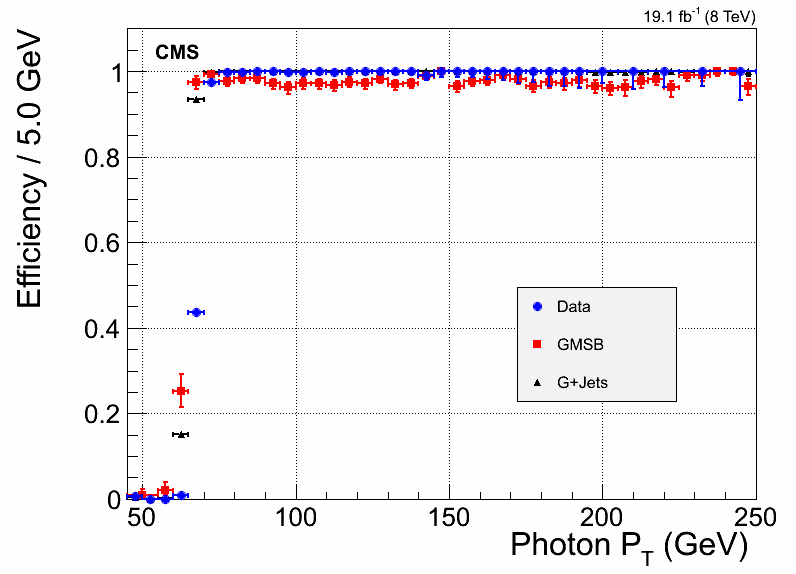
\includegraphics[height=0.45\textwidth,width=0.85\textwidth]{THESISPLOTS/Photon_EffAsym.png}
    \end{column}
    \begin{column}{0.55\linewidth}
     \includegraphics[height=0.45\textwidth,width=0.85\textwidth]{THESISPLOTS/PFMET_EffAsym.png} 
    \end{column}
  \end{columns}
\end{tcolorbox}  
\end{minipage} 
 \begin{minipage}[b]{\linewidth}
   \begin{tcolorbox}[colback=UNL@Cream!5,colframe=UNL@Cream!70,title=\textcolor{UMN@Maroon}{\textbf{}}]
   \includegraphics[height=0.33\textwidth,width=0.70\textwidth]{THESISPLOTS/Eff2D.png}
  \end{tcolorbox} 
 \end{minipage}
\end{frame}

%% Diagram of Why Long-Live Decay Kinematics
\begin{frame}
\frametitle{Delayed Photons}
%\vspace{-1cm}
\begin{minipage}[t]{.85\paperwidth}
  % \begin{varblock}[7cm]{Why Long-Lived?}
  %\setbeamertemplate{itemize items}{$\mathbb{\rhd*}$} %\otimes, \ominus \dagger
   %\begin{itemize}
   \begin{tcolorbox}[colback=UNL@Cream!5,colframe=UNL@Cream!70,title=\textcolor{UMN@Maroon}{\textbf{Source of Delayed Photons? }}]
     %\item \textcolor{UMN@Maroon}{\textbf{Source of Delayed Photons?}}
     \begin{itemize}
      \item Decay of slow moving particles; $\beta << 1$,
      \item Non-nominal photon flight path,
      \item Stopped particles in detector.
      %\item $\cdots$
     \end{itemize}
      \includegraphics[height=0.5\textwidth, width=\linewidth]{THESISPLOTS/DelayedPhoton-ECAL.png}
    \end{tcolorbox}
   \end{minipage}
\end{frame}

%% How to do multicolumns
%% \begin{multicols}{2}
    %\columnbreak
%% \end{multicols}
%Long-Lived Or Offpoint
\begin{frame}
\frametitle{Slow Vs Off-Pointing Decay}
  \begin{minipage}[t]{0.80\paperwidth}
    \begin{columns}
     \begin{column}{0.55\linewidth}
      \begin{tcolorbox}[colback=UNL@Cream!5,colframe=UNL@Cream!70,title=\textcolor{UMN@Maroon}{\textbf{Photon Measured Time}}]
      %\begin{varblock}[3.5cm]{Photon Arrival Time}
          $$\Delta t_{1} = (L1/c\beta) - (L1/c)$$
          $$\Delta t_{2} = (L1 + L2 - L3)/c $$   
           
       %\end{varblock}
        \end{tcolorbox}
      \end{column}
      \begin{column}{0.50\linewidth}
       \begin{tcolorbox}[colback=UNL@Cream!5,colframe=UNL@Cream!70,title=\textcolor{UMN@Maroon}{\textbf{ }}]
           \includegraphics[height=0.5\linewidth, width=0.85\linewidth]{THESISPLOTS/DelayedPhoton-ECAL.png}
       \end{tcolorbox}
      \end{column}
     \end{columns}
  \end{minipage}
  
  \begin{minipage}[b]{0.85\paperwidth}
   \begin{tcolorbox}[colback=UNL@Cream!5,colframe=UNL@Cream!70,title=\textcolor{UMN@Maroon}{\textbf{ }}]
    \includegraphics[height=0.30\linewidth, width=\linewidth]{THESISPLOTS/dt1_dt2_late.png}
    \begin{itemize}
     \item Delayed photons mostly from slow moving decay.    
    \end{itemize}
    \end{tcolorbox}
  \end{minipage}
\end{frame}


%% Decay Kinematics Distribution
\begin{frame}
\frametitle{Kinematic Distribution}
\begin{minipage}[t]{0.83\paperwidth}
  \begin{columns}
     \begin{column}{0.50\linewidth}
       \begin{tcolorbox}[colback=UNL@Cream!5,colframe=UNL@LightGrey!70,title=\textcolor{UMN@Maroon}{\textbf{Photon $p_{T}$ }}]
    \mbox{
           \includegraphics[height=2cm,width=\textwidth]{THESISPLOTS/GMSB_PhotPt.png}}
       \end{tcolorbox}    
     \end{column}
     \begin{column}{0.50\linewidth}
     \begin{tcolorbox}[colback=UNL@Cream!5,colframe=UNL@LightGrey!70,title=\textcolor{UMN@Maroon}{\textbf{Neutralino $c\tau$ }}]
     
     \mbox{
\includegraphics[height=2cm, width=\textwidth]{THESISPLOTS/GMSB_MET.png}}
      \end{tcolorbox}
     \end{column}
   \end{columns}
\end{minipage}
\begin{minipage}[b]{0.83\paperwidth}
 \begin{columns}
     \begin{column}{0.50\linewidth}
      \begin{tcolorbox}[colback=UNL@Cream!5,colframe=UNL@LightGrey!70,title=\textcolor{UMN@Maroon}{\textbf{MET($E^{\mbox{miss}}_{T}$)}}] 
    \mbox{
           \includegraphics[height=2cm,width=\textwidth]{THESISPLOTS/GMSB_MET.png}}
       \end{tcolorbox}    
     \end{column}
     \begin{column}{0.50\linewidth}
     \begin{tcolorbox}[colback=UNL@Cream!5,colframe=UNL@LightGrey!70,title=\textcolor{UMN@Maroon}{\textbf{NJets}}]
     \mbox{
\includegraphics[height=2cm, width=\textwidth]{THESISPLOTS/GMSB_MET.png}}
      \end{tcolorbox}
     \end{column}
   \end{columns}
\begin{itemize}
    \item Different $\Lambda$ values with the same $c\tau$(10~m). Photon $p_{T}$ is harder with higher values of $\Lambda$.
  \end{itemize}
 \end{minipage}
\end{frame}

% Signal Efficiency & Acceptance
\begin{frame}
 \frametitle{Signal Efficiency and Acceptance}

   \begin{minipage}[t]{0.83\paperwidth}
 
  \begin{columns}
     \begin{column}{0.50\linewidth}
       \begin{tcolorbox}[colback=UNL@Cream!5,colframe=UNL@LightGrey!70,title=\textcolor{UMN@Maroon}{\textbf{Efficiency}}]
    \mbox{
           \includegraphics[height=2cm,width=\textwidth]{THESISPLOTS/Eff_ctbgT.png}}
       \end{tcolorbox}    
     \end{column}
     \begin{column}{0.50\linewidth}
     \begin{tcolorbox}[colback=UNL@Cream!5,colframe=UNL@LightGrey!70,title=\textcolor{UMN@Maroon}{\textbf{Acceptance }}]
     
     \mbox{
\includegraphics[height=2cm, width=\textwidth]{THESISPLOTS/Accp_ctbgT.png}}
      \end{tcolorbox}
     \end{column}
   \end{columns}
   \begin{itemize}
    \item Slow moving neutralino decay causes sudden efficiency drop.
   \end{itemize}
\end{minipage}
\begin{minipage}[b]{0.83\paperwidth}
 \begin{columns}
     \begin{column}{0.50\linewidth}
      \begin{tcolorbox}[colback=UNL@Cream!5,colframe=UNL@LightGrey!70,title=\textcolor{UMN@Maroon}{\textbf{Slow moving}}] 
    \mbox{
           \includegraphics[height=2cm,width=\textwidth]{THESISPLOTS/Accp_ctbgT1.png}}
       \end{tcolorbox}    
     \end{column}
     \begin{column}{0.50\linewidth}
     \begin{tcolorbox}[colback=UNL@Cream!5,colframe=UNL@LightGrey!70,title=\textcolor{UMN@Maroon}{\textbf{Off-Pointing}}]
     \mbox{
\includegraphics[height=2cm, width=\textwidth]{THESISPLOTS/Accp_ctbgT2.png}}
      \end{tcolorbox}
     \end{column}
   \end{columns}
\begin{itemize}
    \item Peak Acceptance at transverse decay length= 800~mm.
  \end{itemize}
 \end{minipage}
 
\end{frame}

%% Signal and Bakcground
\begin{frame}
\frametitle{\Huge{Signal and Background}}
\begin{tcolorbox}[colback=UNL@Cream!5,colframe=UNL@LightGrey!70,title=\textcolor{UMN@Maroon}{\textbf{\large{Signal Events}}}]

\end{tcolorbox}

\begin{tcolorbox}[colback=UNL@Cream!5,colframe=UNL@LightGrey!70,title=\textcolor{UMN@Maroon}{\textbf{\large{Background Events}}}]

\begin{itemize}
     \large{
      \item \textbf{Collision}:mis-measured time of $Z/W/top$ events.
      \item \textbf{Non-Collision}:Out-time events from LHC proton Beam/Cosmic/Anomalous Spikes.
      }
 \end{itemize}     
\end{tcolorbox}

     
\end{frame}



%%%Sources of BKG
\begin{frame}
\frametitle{\huge{Non-Collision Background}}
  \begin{minipage}[t]{\paperwidth}
   \begin{itemize}
    \item \textcolor{UMN@Maroon}{\textbf{Background Sources}} 
   
   
  \end{itemize}
 \includegraphics[height=0.45\textwidth, width=0.65\textwidth]{THESISPLOTS/Background_Delayed_Photon.pdf}
  \end{minipage}
% \begin{minipage}[t]{0.8\linewidth}
%  A combination of collision and non-collision events makes up delayed photon background sources.
% \end{minipage}
\end{frame}


%\section{Analysis Strategy}
\begin{frame}
\frametitle{Analysis Strategy}
\begin{itemize}
 \item \textcolor{UMN@Maroon}{\textbf{Strategy}}
   \begin{enumerate}
    \item[I] Identify, tag and reject Non-Collision events.
    \item[II] Perform ABCD background estimation technique on residual non-collision events.
    \item[III]Perform ABCD background estimation technique on collision events.
    \item[IV] Performed a combined ABCD background estimation technique. 
    \end{enumerate}
 \item \textcolor{UMN@Maroon}{\textbf{Clusure Test}}\\
 Verify background estimation methodology by performing a combined ABCD technique on a control sample.
 \item \textcolor{UMN@Maroon}{\textbf{Cross-Check}}\\
 Another check on background estimation of collision events on a separate control sample.
\end{itemize}  
\end{frame}


%%%% Begin Analysis
\begin{frame}
\frametitle{Events Cleaning}
 %\begin{figure}[ht]
  \begin{minipage}[t]{\linewidth}
 \setbeamertemplate{itemize items}[triangle]
  \begin{itemize}
  \item Non-collision events like proton Beam Induced Background~(BIM or     Halos)/Cosmic/Anomalous spikes contribute towards delayed photons ECAL timing. 
  \item Need to defined a cleaning mechanism for identifying and rejecting non-collision events.
  \end{itemize}
  \end{minipage}
  
  \begin{minipage}[t]{\linewidth}
  %\begin{figure}[ht]
    %\centering
 %   \mbox{
 %\includegraphics[width=0.40\paperwidth]{THESISPLOTS/h_Phi_Time.png}
 %includegraphics[width=0.40\paperwidth]{THESISPLOTS/h_Eta_Time.png} }
 \mbox{
 \includegraphics[height=4cm,width=0.40\paperwidth]{THESISPLOTS/SinglePhotonDataSet-TimeVsPhi.pdf}
 \includegraphics[height=4cm,width=0.40\paperwidth]{THESISPLOTS/SinglePhotonDataSet-TimeVsEta.pdf}
 }
    %\vspace{-1cm}
    %\caption{Background}
   \end{minipage}
\begin{minipage}[b]{\linewidth}
Features around $\phi = 0, \pm \pi$ and $\eta$-dependence shows that background sources originate from both collision and non-collision events.
\end{minipage} 
 %\end{figure}
\end{frame}


%% Halo Photon
\begin{frame}
\frametitle{Halo Photon (HP)}
 \begin{tcolorbox}[colback=UNL@Cream!5,colframe=UMN@Maroon!40,title=\textcolor{UMN@Maroon}{\textbf{Beam Halo Muons}}]
\begin{itemize}
 \item Proton beam interacting with gas/air particles in the beam pipe,
 \item Proton beam colliding with the collimators upstream prior to entering the CMS detector.
\end{itemize}
will produce energetic muons traveling parallel with main proton beam and showering in the Calorimeters.
\end{tcolorbox}
 \begin{minipage}[t]{0.8\linewidth}
  \mbox{
   \includegraphics[height=3.7cm,width=0.40\paperwidth]{THESISPLOTS/Beam_Halo-CandidateEvent24186728-Run122314.png}\quad
   \includegraphics[height=3.7cm,width=0.40\paperwidth]{THESISPLOTS/beam_halo_csc.png}
  }   
 \end{minipage}
\end{frame}

%halo Photons
\begin{frame}
\frametitle{Halo Photon (II)}
   \begin{minipage}[t]{\textwidth}
    Using Halo kinematics, We can tag and estimate halo photons produced from halo muons showering in ECAL as follows:
    \begin{columns}
      \column{0.3\textwidth}
      \includegraphics[height=3.0cm,width=0.25\paperwidth]{THESISPLOTS/Halo-Schematic-Diagram.jpg}
      \column{0.60\textwidth}
      %\begin{tcolorbox}[colback=UNL@Cream!5,colframe=UMN@Maroon!40!black,title=Halo Expected Time]
      \begin{varblock}[5.1cm]{\textbf{Halo Expected ECAL Time}}
      %\ovalbox{
      %\begin{bclogo}
      %\begin{itemize}
     % \item \textcolor{UMN@Maroon}{\textbf{Halo Expected ECAL Time}}           
         \begin{eqnarray*}                      
              t_{0} &=& \frac{\rho}{c} = \frac{R}{\sin\theta}\frac{1}{c}, \quad 
              t_{halo} = \frac{Z}{c} = \frac{R}{\tan\theta}\frac{1}{c} \\
              \Delta t^{exp}_{H} &=& t_{halo}- t_{0}=-\frac{R}{2c}\exp^{-\eta}                         
         \end{eqnarray*}              
      %\end{itemize}
      %\end{bclogo}  
        %}      
      \end{varblock}                   
      \end{columns}
   \end{minipage}  
   \begin{minipage}[t]{\linewidth} 
   \mbox{
     \includegraphics[height=3.8cm,width=0.82\paperwidth]{THESISPLOTS/HaloFunction.png}
    }  
   \end{minipage}  
\end{frame}

\begin{frame}
\frametitle{Halo Photon (III)}
 \begin{minipage}[t]{\linewidth}
  Additionally, using halo muon hits from CSC segment matched in $\phi$ to Superclusters in ECAL, we can in additionally identify, tag and remove halo photon events with large timing.
    \begin{columns}
      \column{0.42\textwidth}
         \mbox{
            \includegraphics[height=3cm,width=0.35\paperwidth]{THESISPLOTS/CSC_Beam-Halo-Muon_ev62604_836.png}
          }
      \column{0.55\textwidth}
        \begin{varblock}[4.0cm]{\textbf{Halo Photon Matching}}
          \begin{eqnarray*}
             \Delta \phi (CSC Seg, \gamma) = | \phi_{CSC Seg} - \phi_{\gamma} |
           \end{eqnarray*}
        \end{varblock}     
    \end{columns}
  \end{minipage}
  \begin{minipage}[t]{\linewidth}
  \includegraphics[height=3.6cm,width=0.80\paperwidth]{THESISPLOTS/cs_side_cscdPhi.png} 
   \end{minipage}
\end{frame}


%% Halo Photon Efficiency & Mis-tagging rate
\begin{frame}
\frametitle{Halo Photon (IV)}
 \begin{minipage}[t]{0.85\paperwidth}
   %\begin{columns}
    %\column{0.60\textwidth}
    \begin{tcolorbox}[colback=UNL@Cream!5,colframe=UMN@Maroon!40,title=\textcolor{UMN@Maroon}{ \textbf{Satellite/Ghost Beam Halos}}]
      \begin{itemize}
       \item Fill empty RF buckets.
       \item Trail main bunches by $\approx 5$~ns.
       \item $10^{-5}$ protons compared to main bunches.
       \item Can contribute to main collision photons.
       \item Show a $2.5$~ns pattern in EE,
       \item Tagged using $\Delta\phi(CSC seg, \gamma)$.
      \end{itemize} 
      \end{tcolorbox}
 \end{minipage}
 \begin{minipage}[t]{0.95\paperwidth}
    %\column{0.35\textwidth}  
    %\begin{tcolorbox}[colback=UNL@Cream!5,colframe=UMN@Maroon!40,title=LHC LDM Profile] 
    \centering
    \begin{varblock}[6cm]{LHC LDM Proton Beam Profile}
    \centering
    \mbox{
     \includegraphics[height=2.1cm,width=0.8\linewidth]{THESISPLOTS/Ghost-Satellite-Bunches-LDM.png} 
     }
     %\end{tcolorbox}  
     \end{varblock}  
     %\end{columns}
 \end{minipage}
 
\end{frame}

\begin{frame}
\frametitle{Halo Photon (V)}
 \begin{minipage}[t]{0.85\paperwidth}
  %\begin{columns}
   % \column{0.50\textwidth}
      \begin{tcolorbox}[colback=UNL@Cream!5,colframe=UMN@Maroon!40 ,title=\textcolor{UMN@Maroon}{\textbf{Halo Photon Event Properties}}]
       \begin{itemize}
          \item Halo photons populate around $\phi=0, \pm \pi$
          \item ECAL time mostly $ < -3$~ns but can also arrive late(ghosts).
          \item Halo events most contain no jets ($0$-jet events).
          \item Rare cases can be associated with "pile-up" events.     
       \end{itemize}  
      \end{tcolorbox}
  \end{minipage}
  \begin{minipage}[t]{0.9\paperwidth}
     \begin{columns}
       \column{0.60\textwidth}
        \begin{tcolorbox}[colback=UNL@Cream!5,colframe=UMN@Maroon!40,title=\textcolor{UMN@Maroon}{\textbf{Halo Photon Tagging Criteria}}] 
        \begin{itemize}
         \item Use $\Delta\phi(CSC seg, \gamma) < 0.05$ randians.
         \item Shower shape( $0.8 < S_{Major} < 1.65 $ and $ S_{minor} < 0.2 $)
        \end{itemize}
        \end{tcolorbox}
       \column{0.40\textwidth}
        \begin{varblock}[2.5cm]{Ghost/Satellite EE}
        \centering      
        \includegraphics[height=2.95cm,width=0.29\paperwidth]{THESISPLOTS/halo_EE_Time.png} 
        \end{varblock}
     \end{columns} 
  \end{minipage}   
\end{frame}

%% Cosmic Muons
\begin{frame}
\frametitle{Cosmic Muons}
\small{
% \begin{tcolorbox}[colback=UNL@Cream!5,colframe=UMN@Maroon!40,title=\textcolor{black}{\textbf{Cosmic Muons}}] 
 \begin{varblock}[7cm]{\textbf{Cosmic Muons}}
 \begin{itemize}
  \item Muons from cosmic rays in CMS detector.
  \item Hits in muon detectors~(DT/CSC) and shower in ECAL.
  \item Produce energetic photons with out-of-time.
  \item Using DT segment matched to ECAL cluster position in $\delta \eta$ and $\delta \phi$ can eliminate cosmic events.
 \end{itemize}
 \end{varblock}
 %\end{tcolorbox}
 }
 \vspace{-0.2cm}
%\begin{minipage}[t]{0.9\paperwidth} 
 \begin{tcolorbox}[colback=UNL@Cream!5,colframe=UMN@Maroon!40,title=\textcolor{UMN@Maroon}{$DT(\delta \eta, \delta \phi)$\textbf{Cosmic Muon dataset(left) and Data(Right)}}]
 %\begin{varblock}[7cm]{$DT(\delta \eta, \delta \phi)$\textbf{Cosmic dataset(left) and Data(Right)}}
 \mbox{ 
 \includegraphics[height=2.50cm,width=0.3\paperwidth]{THESISPLOTS/Cosmic_Ray_Photons_Cosmic_dataset.png} \quad \quad
 \includegraphics[height=2.50cm,width=0.3\paperwidth]{THESISPLOTS/cosmics_dPhidEta.png}
 } 
 \end{tcolorbox}
  %\end{varblock}
 %\end{minipage} 
 \vspace{-0.2cm}
 $DT(\delta \eta, \delta \phi)$ tagging of cosmic muons in data and a pure cosmic sample(without LHC proton beam) is comparable.
 
 
\end{frame}

%% Anomalous Events
\begin{frame}
\frametitle{Anomalous ECAL Spike}
 %\begin{minipage}[t]{\paperwidth}
 \small{
% \begin{tcolorbox}[colback=UNL@Cream!5,colframe=UMN@Maroon!40,title=\textcolor{black}{\textbf{Cosmic Muons}}] 
 \begin{varblock}[7cm]{\textbf{ECAL Spikes}}
 \begin{itemize}
  \item Energetic particles(neutrons) from proton collision directly hitting APDs/VPTs.
  \item Associated with hadronic activity.
  \item Observed as photons with early time due to no crystal scintillation.
  \item Can produced late ECAL timing photons with small shower shape.
  \item ID and rejected requiring $1 - \frac{E_{4}}{E_{1}} < 0.9$ of crystal energy deposit and $\chi^{2}$ from pulse shape fitting.
 \end{itemize}
 \end{varblock}
 %\end{tcolorbox}
 }
 \vspace{-0.2cm}
%\begin{minipage}[t]{0.9\paperwidth} 
 \begin{tcolorbox}[colback=UNL@Cream!5,colframe=UMN@Maroon!40,title=\textcolor{UMN@Maroon}{\textbf{Spike Identification and Rejection}}]
 %\begin{varblock}[7cm]{$DT(\delta \eta, \delta \phi)$\textbf{Cosmic dataset(left) and Data(Right)}}
 \mbox{ 
 \includegraphics[height=2.20cm,width=0.3\paperwidth]{THESISPLOTS/seedTime_Chi2.png} \quad \quad
 \includegraphics[height=2.20cm,width=0.3\paperwidth]{THESISPLOTS/swissX.png}
 } 
 \end{tcolorbox}
  %\end{varblock}
 %\end{minipage}
% \end{minipage}
\end{frame}


%%% MET Redefination
\begin{frame}
\frametitle{PF-Missing Transverse Energy(PF-MET)}

\begin{tcolorbox}[colback=UNL@Cream!5,colframe=UMN@Maroon!40,title=\textcolor{UMN@Maroon}{\textbf{PF-Missing Transverse Energy($\ETm$)}}]
Standard PF-MET calculation excludes $\ET$ from out-of-time photons.
We adjusts for this by taking into account the $\ET$ of out-of-time photons in $\ETm$ measurements. This  PF-MET with photon is \textcolor{blue}{ $\METG$}.
  \begin{itemize}
    \item $\mathbf{\ETm}$: PF-MET.
    \item $\mathbf{\METG}$: PF-MET with photon $\ET$.
  \end{itemize}
\end{tcolorbox}

  \begin{tcolorbox}[colback=UNL@Cream!5,colframe=UMN@Maroon!40,title=\textcolor{UMN@Maroon}{\textbf{Signal Selection Criteria}}]
\textcolor{UMN@Maroon}{\textbf{SIGNAL}}: \textcolor{red}{$\geq 1 \gamma$}  + \textcolor{green}{$\geq 2 Jets$} + \textcolor{blue}{$E^{\mbox{miss}}_{T} > 60$~GeV, $\METG > 60$~GeV}
   \end{tcolorbox}
\end{frame}


% Event Selection
%\section{Event Selection}
\begin{frame}
\frametitle{Event Selection}
%\subsection{Pre-Event Selection}
%\subsection{Event Cleaning}
%\subsection{Final Event Selection}
\begin{minipage}[b]{0.45\linewidth}
%\begin{center}
%\begin{table}[ht]
\centering
\small{
\begin{tabular}[2cm]{l l}
\multicolumn{2}{c}{\bfseries{Object Selection Criteria}} \\
  \hline 
  \bfseries{Variable} & \bfseries{Selection Cuts} \\
   \hline 
 % \texttt{primary vertex number of tracks(vnof)}& $>= 4$ \\
 % \texttt{primary vertex transverse distance to beam}~($d0$) & $ < 2$~cm from CMS center \\
%  \texttt{primary vertex longitudinal distance to beam}~($|z|$) & $ < 24$~cm from CMS center \\
  \texttt{Photon} $p_{T}(\gamma^{1(2)})$  & $ > 80(45)$~GeV \\
  %\texttt{Sub-Leading photon must have} $p_{T}(\gamma^{2})$  & $ > 45$~ GeV \\
 $|\eta_{\gamma}|$,(\texttt{EB only}),  &$ < 3.0$($ < 1.5$) \\
 \texttt{Semi-minor axis}($S_{Minor}$)  &$0.12 \leq S_{Minor} \leq 0.38$ \\
 \texttt{H/E}  & $ < 0.05$ \\
 \texttt{Track Vito},$\Delta R(\gamma, track)$  & $ > 0.6 $ \\
 \texttt{HCAL,ECAL, Track, Isolation}  & $ < 4.0 $,$ < 4.5 $,$ < 0.2 $ \\
 \texttt{Cone Size(Iso $\gamma$)} $\Delta R(\gamma, SC)$ & $< 0.4$ \\
 \texttt{Spike Swiss-Cross} & $1-E_{4}/E_{1})< 0.98$ \\ 
 %\texttt{Spike Swiss-Cross} & $1-E_{6}/E_{2} $,($1-E_{4}/E_{1})< 0.98$ \\ 
 % \hline 
%\end{tabular}
%\label{tab:PhotonSel}
%\end{table}
%\end{center}
%%\end{minipage}

%%\begin{minipage}[b]{0.55\linewidth}
%%\begin{center}
%\begin{table}[ht]
%%\centering
%%\begin{tabular}{ll}
%%\multicolumn{2}{c}{\bfseries{PF Jet Selection Criteria}} \\
  \hline 
  \hline
%%  \bfseries{Variable} & \bfseries{Selection Cuts} \\
%%   \hline 
 \texttt{Jets must satisfy} & \texttt{JetID Requirements} \\
 \texttt{Leading Jet} $p_{T}$ & $ > 35$~GeV \\
 \texttt{Number Of Constituents} & $ > 1$ \\
%% \texttt{Charge EM energy fraction~(CEF)}& $ < 0.99$ \\
%% \texttt{Neutral Hadron energy fraction~(NHF)}& $ < 0.99$ \\
%% \texttt{Neutral EM energy fraction~(NEF)}& $ < 0.99$ \\
% \texttt{If} $|\eta|$ \texttt{of jet is} $ >2.4$, \texttt{Charge Hadron energy fraction~(CHF) } & $ > 0$ \\
% \texttt{If} $|\eta|$ \texttt{of jet is} $ >2.4$, \texttt{Charge multiplicity~(NCH) } & $ > 0$ \\
 $\Delta R(\gamma, jet) = \sqrt{(\phi_{\gamma}-\phi_{jet})^{2} + (\eta_{\gamma}-\eta_{jet})^{2}}$ & $ > 0.3$ \\
\hline \hline
 $\ETm$&  $> 25$~GeV \\
 \hline
\end{tabular}
}
  \end{minipage}
\end{frame}



 %% Mis Tagg Rate and Bkg Estimation
 \begin{frame}
\frametitle{Mis-Tagging Rate}
 \begin{minipage}[t]{0.8\paperwidth}
   \begin{itemize}
    \item Tagging reliable but not 100\% efficient.
   \end{itemize}

  \begin{columns}
   \column{0.45\linewidth}
    \begin{tcolorbox}[colback=UNL@Cream!5,colframe=UMN@Maroon!40,title=Mis-Tag Rates]
     \begin{tabular}{|| c|c||}
        %\multicolumn{2}{c}{\bfseries{Mis-Tag Rates}} \\
        \multicolumn{2}{c}{\bfseries{}} \\
        \hline 
         \texttt{Halo} & $\approx 5$\% \\       
          \hline \hline
         \texttt{Cosmic}& $\approx 6$\% \\
          \hline \hline   
         \texttt{Spike} & $\approx 1.5$\% \\
        \hline
        \end{tabular} 
    \end{tcolorbox}
 \column{0.60\linewidth}
 \begin{tcolorbox}[colback=UNL@Cream!5,colframe=UMN@Maroon!40,title=Tagging Performance]
 
    \includegraphics[height=5.5cm,width=0.40\paperwidth]{THESISPLOTS/TimeForAll.png}
    
 \end{tcolorbox}
  \end{columns}
   \end{minipage}
\end{frame}





%% Here we Estimate Background.
%\section{Background Estimation}
\begin{frame}
\frametitle{ABCD Background Estimation}
\small{
After tagging and cleaning Halo/Cosmic/Spike events, We apply \alert{ABCD} background estimation technique on residual Non-collision background events to estimate their contribution to possible signal.}
\begin{tcolorbox}[colback=UNL@Cream!5,colframe=UMN@Maroon!40,title=\textcolor{UMN@Maroon}{\textbf{Event Tagging and Cleaning Performance}}]

\mbox{
 \includegraphics[height=4.5cm,width=0.99\linewidth]{THESISPLOTS/TimeForAll.png}
 } 
 \end{tcolorbox}
\end{frame}

\begin{frame}
\frametitle{ABCD Method: Non-Collision Background}
 \begin{minipage}[t]{0.8\paperwidth}
%\begin{tcolorbox}[colback=UNL@Cream!5,colframe=UMN@Maroon!40,title=\textcolor{black}{\textcolor{blue}{\textbf{Assume similar distribution in ECAL time for untagged non-collision events .}}}]
\begin{tcolorbox}[colback=blue!5,colframe=UMN@Gold!40,title=\textcolor{UMN@Maroon}{\textcolor{UMN@Maroon}{\textbf{Non-Collision Events.}}}]
  %\begin{varblock}[7.2cm]{\textbf{Non-Collision Events.}}
  
      \centering
        \begin{tabular}{|c || c|| c|}
        \multicolumn{3}{c}{\bfseries{$\ETm > 60$~GeV}} \\
        \hline 
          & $\METG < 60$ & $\METG > 60$ \\       
          \hline \hline
          $-10 < t < -3$~ns & A &  B \\
          \hline \hline   
          $3 < t < 13$~ns & C &  D \\
        \hline \hline
        \end{tabular} 
  %\end{varblock}
\end{tcolorbox}
\end{minipage}
\begin{minipage}[b]{.8\paperwidth} 
  \begin{columns}
   \begin{column}{0.55\linewidth}
     \includegraphics[height=4.0cm,width=0.99\linewidth]{THESISPLOTS/TimeForAll.png} 
   \end{column}
  \begin{column}{0.45\linewidth}
  
      $\frac{D}{C} = \frac{B}{A}, \Rightarrow $
      
      \begin{tcolorbox}[colback=blue!5,colframe=UMN@Gold!40]
         \begin{equation*}
           \mathbf{D = \frac{B}{A}\cdot C }
         \end{equation*}
     \end{tcolorbox}
     \end{column}
    \end{columns}
\end{minipage}
\end{frame}

% ABCD Collision
\begin{frame}
\frametitle{ABCD Method: Collision Background}
 \begin{minipage}[t]{0.8\paperwidth}
%\begin{tcolorbox}[colback=UNL@Cream!5,colframe=UMN@Maroon!40,title=\textcolor{black}{\textcolor{blue}{\textbf{Assume similar distribution in ECAL time for untagged non-collision events .}}}]
  %\begin{varblock}[7.2cm]{\textbf{Collision Events.}}
    \begin{tcolorbox}[colback=blue!5,colframe=UMN@Gold!40,title=\textcolor{UMN@Maroon}{\textcolor{UMN@Maroon}{\textbf{Collision Events.}}}]
   %\begin{columns}
     %\column{0.65\linewidth}
      \centering
        \begin{tabular}{|c || c|| c|}
        \multicolumn{3}{c}{\bfseries{$\METG < 60$~GeV}} \\
        \hline \hline
          & $ \ETm < 60$ & $ \ETm > 60$ \\       
          \hline \hline
          $-10 < t < -3$~ns & $B^{\prime}$ &  B \\
          \hline \hline \hline    
          $ |t| < 2$~ns & $F^{\prime}$ &  $F$ \\
          \hline \hline \hline
          $ 3 < t > 13$~ns & $D^{\prime}$ &  $D$ \\
        \hline \hline
        \end{tabular} 
     %\column{0.26\linewidth}
    %\end{columns}
 \end{tcolorbox}   
%\end{varblock}
%\end{tcolorbox}
\end{minipage}
\begin{minipage}[b]{0.8\paperwidth} 
  \begin{columns}
   \begin{column}{0.55\linewidth}
    \includegraphics[height=3.4cm,width=0.99\linewidth]{THESISPLOTS/TimeForAll.png}
  \end{column}
  \begin{column}{0.45\linewidth}
        $\frac{D}{D^{\prime}} = \frac{F}{F^{\prime}}, \frac{B}{B^{\prime}} = \frac{F}{F^{\prime}} \Rightarrow$
      \begin{tcolorbox}[colback=blue!5,colframe=UMN@Gold!40]
        \begin{equation*}
          \mathbf{Q_{d} = \frac{F}{F^{\prime}}\cdot D^{\prime} }
         \end{equation*}
         \begin{equation*}
           \mathbf{Q_{b} = \frac{F}{F^{\prime}}\cdot B^{\prime} }
         \end{equation*}
     \end{tcolorbox}   
  \end{column}
 \end{columns}
 \end{minipage}
\end{frame}

% ABCD Combined 
\begin{frame}
\frametitle{ABCD Method:Combined Background}
 \begin{minipage}[t]{0.8\paperwidth}
    \begin{tcolorbox}[colback=blue!5,colframe=UMN@Gold!40,title=\textcolor{UMN@Maroon}{\textbf{Combined Background Estimation.}}]
         \begin{equation*}
           \mathbf{D = \frac{B- Q_{b} }{A}\cdot C + Q_{d} }
         \end{equation*}
     \end{tcolorbox}
 \end{minipage}
 
 \begin{minipage}[b]{0.8\paperwidth}
  \begin{tcolorbox}[colback=UNL@Cream!5,colframe=UMN@Maroon!40,title=\textcolor{UMN@Maroon}{\textbf{Closure Test: $< 2$-Jets Events}}]
     %\begin{columns}
      %\begin{column}{0.65\linewidth}
      \begin{tabular}{|c || c|| c|}
        \multicolumn{3}{c}{\bfseries{$\METG < 60$~GeV}} \\
        \hline \hline
          & $ \ETm < 60$ & $ \ETm > 60$ \\       
          \hline \hline \hline
          $-10 < t < -3$~ns & $B^{\prime}$ &  B \\
          \hline \hline \hline    
          $ |t| < 2$~ns & $F^{\prime}$ &  $F$ \\
          \hline \hline \hline
          $ 3 < t > 13$~ns & $D^{\prime}$ &  $D$ \\
        \hline \hline \hline
       \end{tabular}
     \end{tcolorbox}       
  \end{minipage}
\end{frame}   
   
     %\end{column}
     %\begin{column}{0.35\linewidth} 
\begin{frame}     
  \begin{minipage}[b]{0.8\paperwidth}
   \begin{tcolorbox}[colback=UNL@Cream!5,colframe=UMN@Maroon!40,title=\textcolor{UMN@Maroon}{\textbf{Closure Test: $< 2$-Jets Events}}] 
        \begin{tabular}{|c || c|| c|}
       \multicolumn{3}{c}{\bfseries{$\ETm > 60$~GeV}} \\
       \hline \hline
          & $\METG < 60$ & $\METG > 60$ \\       
          \hline \hline \hline
          $-10 < t < -3$~ns & A &  B \\
          \hline \hline \hline  
         $3 < t < 13$~ns & C &  D \\
        \hline \hline
        \end{tabular}
      %\end{column}
    %\end{columns}  
   \end{tcolorbox} 
 \end{minipage}
 \end{frame}



\begin{frame}
\frametitle{Background Estimation Cross-Check}
 \begin{minipage}[t]{0.8\linewidth}
  \begin{tcolorbox}[colback=UNL@Cream!5,colframe=UMN@Maroon!40,title=\textcolor{UMN@Maroon}{\textbf{ Control Sample $Z\rightarrow ee$ Events}}]
 
 
   \end{tcolorbox}
  \end{minipage}
\end{frame}






%%Systematic Uncertainties
%\section{Systematics}
\begin{frame}
\frametitle{ Systematics}
 \begin{minipage}[t]{0.8\linewidth}
  Background estimation is Data driven.
  Thus, most of a systematics come from signal,including:
  \begin{varblock}[7cm]{Experimental Systematics}
   \begin{itemize}
    \item Definition of Absolute or Zero time,
    \item ECAL time Resolution,    
    \item Unclustered Energy,
    \item Jet energy scale,
    \item Jets energy resolution,
    \item Photon energy scale,
    \item Luminosity. We use standard CMS luminosity uncertainty.
   \end{itemize}
  \end{varblock}  
  \begin{varblock}[7cm]{Theoretical Systematics}
   \begin{itemize}   
   \item Choice of PDF.
   \item Re-normalization group equations.
   \end{itemize}
  \end{varblock} 
\end{minipage}
\end{frame}

\begin{frame}
\frametitle{ Systematics(II)}
\begin{minipage}[t]{0.8\textwidth}
\centering
\begin{tabular}{l l}
  \multicolumn{2}{c}{\bfseries{Systematic Uncertainties}} \\
  \hline 
   \bfseries{Source} & \bfseries{Uncertainty(\%)} \\
   \hline
   \texttt{Absolute time(Zero time)}& $10\sim 6$  \\
   \texttt{Unclustered Energy}&  $10 \sim 4 $  \\
   \texttt{Photon Energy Scale}& $ 4 \sim 2$  \\
   \texttt{ECAL Time Resolution}& $ 5 \sim 2 $   \\
   \texttt{Jet Energy Scale}& $9 \sim 3$   \\
   \texttt{Jet Energy Resolution}& $ 9 \sim 2 $  \\
   \hline
   \texttt{Luminosity} & 2.6    \\
   \texttt{Choice of PDF} & $ < 1$ \\
  \hline \hline
 \end{tabular} 
 \end{minipage}
 
 \begin{minipage}[b]{0.8\textwidth}
 \begin{itemize}
  \item We obtained our systematics by studying the effects of varying by a few amount of a particular source of systematic on the total number of objects passing object selection cuts.
   \end{itemize}
 \end{minipage}
\end{frame}




%Results
\section{RESULTS}
{
\usebackgroundtemplate{%
\tikz\node[opacity=0.35] {\includegraphics[height=\paperheight,width=\paperwidth]{/home/tensr/Documents/TEN-HEP-PHD-THESIS/PHD_THESIS/PHD/PLOTS/CMS_DET.png}};}
\begin{frame}
  \begin{center}
   \textcolor{UMN@Maroon}{\Huge{\textbf{RESULTS}}}
  \end{center}
\end{frame}
}

\begin{frame}
\frametitle{Results}
\begin{minipage}[t]{0.8\textwidth}
\begin{itemize}
 \item Observed \textcolor{UMN@Gold}{\textbf{1 Event}}
 \item Expected \textcolor{UMN@Maroon}{\textbf{0.0886 Events}}
\end{itemize}
\centering
\begin{tabular}{l l l}
\multicolumn{3}{c}{\bfseries{Events Passing Final Selection}} \\
  \hline
   \bfseries{Sample} &\bfseries{Lifetime($c\tau$)[mm]} &\bfseries{Number Of Events} \\
   \hline
   \texttt{GMSB $\Lambda=180$ TeV}& $10500$ & \\
   \texttt{GMSB $\Lambda=180$ TeV}& $ 6000$ &  \\
   \texttt{GMSB $\Lambda=180$ TeV}& $ 4000$&  \\
   \texttt{GMSB $\Lambda=180$ TeV}& $ 3000 $&   \\
   \texttt{GMSB $\Lambda=180$ TeV}& $ 2000$&   \\
   \texttt{GMSB $\Lambda=180$ TeV}& $ 1000$&  \\
   \texttt{GMSB $\Lambda=180$ TeV}& $ 500$&  \\
   \hline
   \texttt{Data} & 1.00 &    \\
   \texttt{Background Total} & $0.0886$ & \\
  \hline \hline
 \end{tabular} 
 \end{minipage}
\end{frame}

%% Observed Event Display
\begin{frame}
\frametitle{Observed Event}
\begin{tcolorbox}[colback=UNL@Cream!5,colframe=UNL@LightGrey!40,title=\textcolor{UMN@Maroon}{\textbf{3-D View}}]
 \centering
\mbox{
\includegraphics[height=3cm,width= 0.7\paperwidth]{THESISPLOTS/Delayed_photon-Event-3D.png}} 
 \end{tcolorbox}
 
 \begin{tcolorbox}[colback=UNL@Cream!5,colframe=UNL@LightGrey!40,title=\textcolor{UMN@Maroon}{\textbf{Transverse~(left) and $\rho-Z$ (Right) View}}]
 \centering
\mbox{
\includegraphics[height=2.5cm,width=0.35\paperwidth]{THESISPLOTS/Delayed_photon_Event-Rho-Phi.png}
 \quad
\includegraphics[height=2.5cm,width=0.35\paperwidth]{THESISPLOTS/Delayed_photon_Event-Rho-Z.png}
} 
 \end{tcolorbox}

\end{frame}

\begin{frame}
\frametitle{Exclusion Limits}
\begin{figure}[ht]
\begin{minipage}[b]{0.45\linewidth}
\centering
\mbox{
\includegraphics[height=6cm,width=\textwidth]{THESISPLOTS/Neutralino_CrossSecTimesBR_Uplimit.pdf}}
\vspace{-1cm}
\caption{$c\tau$ Limits }
\label{fig:ctaulimit}
\end{minipage}
\hspace{0.1cm}
\begin{minipage}[b]{0.45\linewidth}
\centering
\mbox{
\includegraphics[height=6cm, width=\textwidth]{THESISPLOTS/Neutralino_CrosSecVsMass_Exclusion_limit_11000.pdf}}
\vspace{-1cm}
\caption{Mass Limit }
\label{fig:masslimit}
\end{minipage}
\end{figure}
%\vspace{-1cm}
%\alert{\textbf{sample is $c\tau= 12000$ mm but we measure $c\tau \approx 10500$ mm}}
\end{frame}

\begin{frame}
\frametitle{$c\tau$-mass Limits}
 \begin{minipage}[t]{0.8\linewidth}
 %    \centering
      \includegraphics[height= 8cm,width=0.8\paperwidth]{THESISPLOTS/Neutralino_Ctau-Vs-Lambda_2D_exclusion.pdf}
%   \end{minipage}
% \begin{minipage}[t]{\linewidth}
% \newline \textcolor{blue} {\texttt{Y. Kats et al: arXiv:1110.6444v2}}
 \end{minipage}
\end{frame}

%%% Previous Experiments
\begin{frame}
\frametitle{Comparison To Other Search Experiments}
\begin{minipage}[t]{0.82\paperwidth}
 %\begin{tcolorbox}[colback=UNL@Cream!5,colframe=UNL@Cream!40,title=\textcolor{UMN@Maroon}{\textbf{ATLAS}}]
  \setbeamertemplate{itemize items}{$\mathbb{\rhd*}$} %\otimes, \ominus \dagger etc
 \begin{itemize}
  \item \textcolor{UMN@Maroon}{\textbf{ATLAS}}
  %\begin{varblock}[7cm]{\textbf{ATLAS}}
  \includegraphics[height=0.35\textwidth,width=0.90\linewidth]{THESISPLOTS/ATLAS_Upper_Limit.png}

  %\end{varblock}
  %\end{tcolorbox}
 \end{itemize}
\end{minipage}
\begin{minipage}[b]{0.82\paperwidth}
%\begin{tcolorbox}[colback=UNL@Cream!5,colframe=UNL@Cream!40,title=\textcolor{UMN@Maroon}{\textbf{CMS, CDF, DO}}]
 \setbeamertemplate{itemize items}{$\mathbb{\rhd*}$} %\otimes, \ominus \dagger etc
\begin{itemize}
  \item \textcolor{UMN@Maroon}{\textbf{CMS 8 TeV}}
   %\begin{varblock}[7cm]{\textbf{CMS, CDF, DO}}
\includegraphics[height=0.35\textwidth,width=0.90\linewidth]{THESISPLOTS/Neutralino_Ctau-Vs-Lambda_2D_exclusion.pdf}

 %\end{tcolorbox}
 %\end{varblock}
  \end{itemize}
\end{minipage}
\end{frame}





\section{SUMMARY}
{
\usebackgroundtemplate{%
\tikz\node[opacity=0.35] {\includegraphics[height=\paperheight,width=\paperwidth]{/home/tensr/Documents/TEN-HEP-PHD-THESIS/PHD_THESIS/PHD/PLOTS/CMS_DET.png}};}
\begin{frame}
  \begin{center}
    \textcolor{UMN@Maroon}{\Huge{\textbf{SUMMARY}}}
  \end{center}
\end{frame}
}

\begin{frame}
\frametitle{Summary}
\begin{itemize}
\item Discuss Motivation for New Physics.
\item Discuss ECAL Timing.
\item Discuss Search for Long-Lived Particles using ECAL Time.
\item Looking forward to LHC Run II Results on this Analysis.
\end{itemize}
\end{frame}





%%% Thank you Page
{
\usebackgroundtemplate{%
\tikz\node[opacity=0.35] {\includegraphics[height=\paperheight,width=\paperwidth]{/home/tensr/Documents/TEN-HEP-PHD-THESIS/PHD_THESIS/PHD/PLOTS/CMS_DET.png}};}
\begin{frame}
 \begin{center}
   \textcolor{UMN@Maroon}{\Huge{\textsl{Merci Beaucoup!}} }
 \end{center}
 
 \begin{minipage}[b]{0.65\textwidth}
\mbox{
\includegraphics[height=0.65\textwidth,width=0.65\textwidth]{/home/tensr/Documents/TEN-HEP-PHD-THESIS/PHD_THESIS/PHD/THESISPLOTS/darkMatter_Particle.jpg} \quad \quad
\includegraphics[height=0.65\textwidth,width=0.65\textwidth]{THESISPLOTS/New-Physics-PLOTS/ElusiveParticles.png}
}
 \end{minipage}
\end{frame}
}


%%% Back-Up
{
\usebackgroundtemplate{%
\tikz\node[opacity=0.35] {\includegraphics[height=\paperheight,width=\paperwidth]{/home/tensr/Documents/TEN-HEP-PHD-THESIS/PHD_THESIS/PHD/PLOTS/CMS_DET.png}};}
\begin{frame}
  \begin{center}
   \textcolor{UMN@Maroon}{\Huge{\textbf{BACK UP}} }
  \end{center}
\end{frame}
}

\begin{frame}
\frametitle{Funny Quarks}
 \includegraphics[height=0.65\textwidth,width=0.65\textwidth]{THESISPLOTS/New-Physics-PLOTS/FunnyQuarks.jpg}
\end{frame}

%% 2 dim Efficiency
\begin{frame}
\frametitle{Signal Efficiency and Acceptance(III)}
  \begin{figure}[ht]
   \begin{minipage}[b]{0.7\linewidth}
    \mbox{
  \centering
  \includegraphics[height=7.5cm, width=0.65\paperwidth]{THESISPLOTS/Eff180_xPt_ct.png} }
    \vspace{-0.5cm}
    \caption{2 Dim Efficiency}
  \end{minipage}
 \end{figure}
\end{frame}

%%% Control Samples for BKG Estimation
\begin{frame}
\frametitle{Background Control Samples}
We estimate these background by defining two Control samples.
\begin{flushleft}
 \begin{description}
   \item[In-time] events Control Sample~(IT-CS)
   \item[Out-of-time] events Control Sample (OT-CS)
 \end{description} 
 \end{flushleft}
\begin{tcolorbox}[colback=UNL@Cream!5,colframe=UMN@Maroon!40,title=\textcolor{UMN@Gold}{\textbf{Control Sample (In-time Events)}}]
%\lipsum[2]
\textbf{IT-CS}: $> 2$ Jets Events with photon ECAL time, $t \in [-1, 1]$~ns.
\end{tcolorbox}

\begin{tcolorbox}[colback=UNL@Cream!5,colframe=UMN@Maroon!40,title=\textcolor{UMN@Gold}{\textbf{Control Sample (Out-Of-time Events)}}]
%\lipsum[2]
\textbf{OT-CS}: $0$ Jet Events with photon ECAL time, $ t < -3$~ns or $t > 2$~ns.
\end{tcolorbox}
 
 \begin{minipage}[t]{0.8\linewidth}
 Events from above CSs provide a unique approach to estimate possible background contribution in signal.
 \end{minipage}
\end{frame}


%%% Tagging Efficiency
\begin{frame}
\frametitle{HP Tagging Criteria}
  %\begin{columns}
   %\column{0.50\textwidth}
   \begin{minipage}[t]{\linewidth}
     \begin{tcolorbox}[colback=UNL@Cream!5,colframe=UMN@Maroon!40,title=\textcolor{UMN@Maroon}{\textbf{Halo Photon Tagging Efficiency}}]
        \begin{itemize}
         \item Control Sample Selection,
           \begin{itemize}
            \item $\Delta\phi(CSC seg, \gamma) < 0.05$ radians
            \item Same $ \Delta t^{exp}_{H}= -\frac{R}{2c}\exp^{-\eta} $ ECAL time Vs $\eta$ dependence.
           \end{itemize}
         \item Efficiency evaluated in 5$\eta$ bins for $S_{Major}$ $\eta$ dependence.
        \end{itemize}
      \end{tcolorbox} 
   \end{minipage}
   \begin{minipage}[t]{\linewidth} 
    %\column{0.50\textwidth}
     \begin{tcolorbox}[colback=UNL@Cream!5,colframe=UMN@Maroon!40,title=\textcolor{UMN@Maroon}{\textbf{Halo Photon mis-Tag Rate}}]
      \begin{itemize}
         \item Control Sample Selection:
           \begin{itemize}
            \item $ >= 2$-jets events with $E^{miss}_{T} < 60$~GeV
            \item ECAL time, $|t| < 1$~ns.
           \end{itemize}
          \item mis-tag rate eveluated in 5$\eta$ bins for $S_{major}$ $\eta$ dependence.         
        \end{itemize}
      \end{tcolorbox}
  %\end{columns}
  \end{minipage}
\end{frame}




\begin{frame}
\frametitle{HP Tagging Efficiency/mis-Tag Rate(I)}
\begin{columns}
   \column{0.50\linewidth}
%\begin{tcolorbox}[colback=UNL@Cream!5,colframe=UMN@Maroon!40,title=Tagging Efficiency]
 \begin{varblock}[3.5cm]{Tagging Efficiency}
 \includegraphics[height=6.5cm,width=0.40\paperwidth]{THESISPLOTS/Efficiency_Halo.png}
 \begin{itemize}
  \item Tagging Efficiency $\approx 98$\%
 \end{itemize}
 \end{varblock}
 %\end{tcolorbox}
 \column{0.50\linewidth}
 %\begin{tcolorbox}[colback=UNL@Cream!5,colframe=UMN@Maroon!40,title=mis-Tag Rate]
 \begin{varblock}[3.5cm]{mis-Tag Rate}
\includegraphics[height=6.5cm,width=0.40\paperwidth]{THESISPLOTS/MisTagging_Halo.png}
 \begin{itemize}
  \item mis-tag rate $\approx 3$\%
 \end{itemize}
 \end{varblock}
 %\end{tcolorbox}
  \end{columns}
\end{frame}


%Why New Physics?
%New Physics Observation
\begin{frame}
\frametitle{New Physics Everywhere: Observation}
 %\textbf{Expecting New Physics?}
 \vspace{-0.1cm}
\begin{minipage}[b]{0.90\linewidth}
   \begin{tcolorbox}[colback=UNL@Cream!5,colframe=UNL@Cream!60,title=\textcolor{UMN@Maroon}{\textbf{AMS Experiment on ISS}}]
       \mbox{
            \includegraphics[height=0.40\linewidth,width=0.45\linewidth]{THESISPLOTS/New-Physics-PLOTS/AMS-ON-ISS.jpg} \quad \quad 
           \includegraphics[height=0.40\linewidth,width=0.60\linewidth]{THESISPLOTS/New-Physics-PLOTS/AMS-Electron-Positron-Flux-Difference.png} \quad
}
   \end{tcolorbox}
\end{minipage}
 
 
\begin{minipage}[t]{0.80\paperwidth}
\vspace{-0.1cm}
  \begin{columns}
    \begin{column}{0.50\linewidth}
        \begin{tcolorbox}[colback=UNL@Cream!5,colframe=UNL@Cream!60,title=\textcolor{UMN@Maroon}{\textbf{$ZZ$, $WW$ Production}}]     
            \mbox{\includegraphics[height=0.40\linewidth,width=\linewidth]{THESISPLOTS/New-Physics-PLOTS/SigmaR_v5.pdf}}            
         \end{tcolorbox}
   \end{column} 
   
   \begin{column}{0.50\linewidth}
         \begin{tcolorbox}[colback=UNL@Cream!5,colframe=UNL@Cream!60,title=\textcolor{UMN@Maroon}{\textbf{Neutrino Masses.}}]
   
          \includegraphics[height=0.40\linewidth,width=\linewidth]{THESISPLOTS/New-Physics-PLOTS/neutrino-Mass.png}
         \end{tcolorbox}     
      \end{column} 
  \end{columns}
\end{minipage}
\end{frame}

% More New Physics
\begin{frame}
\frametitle{New Physics Everywhere: Observation}
\begin{minipage}[t]{0.80\paperwidth}
 \begin{tcolorbox}[colback=UNL@Cream!5,colframe=UNL@Cream!60,title=\textcolor{UMN@Maroon}{\textbf{Dark Matter.}}]
    \mbox{ 
       \includegraphics[height=0.40\linewidth,width=0.5\linewidth]{THESISPLOTS/New-Physics-PLOTS/DMRotationcurve.jpg}          
       \includegraphics[height=0.40\linewidth,width=0.5\linewidth]{THESISPLOTS/New-Physics-PLOTS/DM-Rotation-Curves.png} 
          }\\
     \mbox{            
\includegraphics[height=0.35\linewidth,width=0.5\linewidth]{THESISPLOTS/New-Physics-PLOTS/7Years_WMAP_CMB.png} \\
 \includegraphics[height=0.35\linewidth,width=0.5\linewidth]{THESISPLOTS/New-Physics-PLOTS/CMB_Multiple_Moments.png} 
 } 
\end{tcolorbox}
\end{minipage}
\end{frame}


\begin{frame}
\frametitle{New Physics Everywhere: Observation}
\begin{minipage}[b]{0.80\paperwidth}
 \begin{tcolorbox}[colback=UNL@Cream!5,colframe=UNL@Cream!60,title=\textcolor{UMN@Maroon}{\textbf{Universe Matter Budget.}}]
\mbox{
\includegraphics[height=0.35\linewidth,width=0.50\linewidth]{THESISPLOTS/New-Physics-PLOTS/UniversePie30.jpg} }
    %\textcolor{UMN@Maroon}{\textbf{Dark Matter Candidate}
   
 \end{tcolorbox}
 
\end{minipage}

\begin{minipage}[b]{0.80\paperwidth}
 \begin{tcolorbox}[colback=UNL@Cream!5,colframe=UNL@Cream!60,title=\textcolor{UMN@Maroon}{\textbf{Dark Matter in our Galaxy?.}}]
 \mbox{
    \includegraphics[height=0.30\linewidth,width=0.50\linewidth]{THESISPLOTS/New-Physics-PLOTS/X-ray-Signature-DM-2014.png}
      }
 \end{tcolorbox}
 
 \end{minipage}
\end{frame}

\end{document}

%%%-------------------------------------------------------------------------------------
%\begin{itemize}
%\begin{large}
%\item Offset in neutralino $c\tau$ seems to have a more subtle origin than expected. Probably how mass enters into the lifetime definition and implementation at MC generation level.
%\item GMSB samples with the same sample $c\tau$, hence $C_{grav}$, but with different $\Lambda$ values have different offset factor.
%\item The observation that the $c\tau$ value for a given sample with $\Lambda$ is different from the measured value is very unclear, even without looking at samples with different $\Lambda$ values.
%\item Our next step involves understanding cause of this offset.
%However,due to time constraints, we might continue with upper limit setting considering this difference.
%\end{large}
%\end{itemize}
%others
%\begin{frame} %---------------------------------------------------------------
%\frametitle{Are these measurements correct?}
% \framesubtitle{}
%\begin{LARGE}
%\textbf{Are we measuring the original $c\tau$ of the neutralino?}
%\end{LARGE}
%\vspace{-0.5cm}
%\begin{table}
%\begin{minipage}[b]{1.0\linewidth}
%\centering
%\begin{tabular}{|l||l||l||l|l|l|}
%\hline
%\multicolumn{5}{|c|}{\bfseries{CMS Official GMSB Samples}} \\
%\hline
%\bfseries{$\Lambda$[TeV]} & \bfseries{mass[GeV]} & \bfseries{$C_{grav}$} & \bfseries{c$\tau$[mm]} & \bfseries{Fit Value[mm]} \\
%\hline
%120 & 169 & 93.5 & 1000 & 657.89 \\
%120 & 169 & 162 & 3000 &1942.12 \\
%\hline
%\hline
%140 & 198 & 162 & 3000 & 1550.38 \\
%140 & 198 & 187 & 4000 & 2064.83 \\
%140 & 198 & 229 & 6000 & 3083.56 \\
%\hline
%\hline
%180 & 256 & 93.5 & 1000 & 378.64 \\
%180 & 256 & 132 & 2000 & 749.45 \\
%180 & 256 & 162 & 3000 & 1104.85 \\
%180 & 256 & 229 & 6000 & 2203.61 \\
%\hline
%\end{tabular}
%\end{minipage}
%\end{table}
%\vspace{-0.5cm}
%\alert{\textbf{We seem to be measuring neutralino $c\tau$ by some factor off.}}
%\end{frame}
%\begin{frame}
%--------------------------------------------------------------------
%\frametitle{GMSB Sample $c\tau$ Vs Measured $c\tau$}
%\begin{LARGE}
%\textbf{By how much are we off in neutralino $c\tau$ measurements?}
%\end{LARGE}
%\begin{table}
%\begin{minipage}[b]{1.0\linewidth}
%\centering
%\begin{tabular}{|l||l||l||l|}
%\hline
%\multicolumn{4}{|c|}{\bfseries{CMS Official GMSB Samples}} \\
%\hline
%\bfseries{$\Lambda$[TeV]} & \bfseries{c$\tau$[mm]} & \bfseries{Fit Value[mm]} &\bfseries{Factor Off} \\
%\hline
%120 & 3000 & 1942.12 & 1.54 \\
%140 & 3000 & 1550.38 & 1.93 \\
%180 & 3000 & 1104.85 & 2.71 \\
%\hline
%\hline
%140 & 6000 & 3083.56 & 1.9 \\
%180 & 6000 & 2203..61 & 2.7 \\
%\hline
%\end{tabular}
%\end{minipage}
%\end{table}
%\vspace{-0.5cm}
%Factor is \alert{The SAME} for different neutralino $c\tau$ with same $\Lambda$ value. However, factor is \alert{NOT THE SAME} for the same $c\tau$ with different $\Lambda$ values.
%\end{frame}
%\begin{frame}
%---------------------------------------------------------------------
%\frametitle{Cause of this difference in $c\tau$ values?}
%\begin{LARGE}
%\textbf{Is this due to how sample is generated?}
%\end{LARGE}
%\vspace{-0.3cm}
%\begin{figure}[ht]
%\begin{minipage}[b]{0.45\linewidth}
%\centering
%\mbox{
%\includegraphics[height=2.5cm, width=\textwidth]{MC_TimeDL.png}}
%\vspace{-1cm}
%\caption{1/Slope = 3083.56 mm }
%\label{fig:OffFrom_MC}
%\end{minipage}
%\hspace{0.1cm}
%\begin{minipage}[b]{0.45\linewidth}
%\centering
%\mbox{
%\includegraphics[height=2.5cm,width=\textwidth]{Priv_MC_TimeDL.png}}
%\vspace{-1cm}
%\caption{1/Slope = 3067.48 mm }
%\label{fig:Priv_MCTime}
%\end{minipage}
%\end{figure}
%\vspace{-1.0cm}
%\begin{figure}[ht]
%\begin{minipage}[b]{0.45\linewidth}
%\centering
%\mbox{
%\includegraphics[height=2.5cm, width=\textwidth]{Dist_TravDL.png}}
%\vspace{-1cm}
%\caption{1/Slope = 3065.60 mm }
%\label{fig:Off_DL}
%\end{minipage}
%\hspace{0.1cm}
%\begin{minipage}[b]{0.45\linewidth}
%\centering
%\mbox{
%\includegraphics[height=2.5cm,width=\textwidth]{Priv_DistTravDL.png}}
%\vspace{-1cm}
%\caption{1/Slope = 3037.66 mm }
%\label{fig:Priv_DL}
%\end{minipage}
%\end{figure}
%\vspace{-1.0cm}
%\alert{\textit{Private GMSB sample seems to show same offset measurements}}
%\end{frame}
%\begin{frame}
%\frametitle{Introduction}
%\begin{varblock}[7cm]{Hybrid Linear Modeling}
%Suppose $\textbf{X} = \left( \mathbf{x}_{1}, \cdots, \mathbf{x}_{N} \right)$.
%sampled from a mixture of $\kappa$ subspaces or flats with dimension $d$
%\end{varblock}
%\begin{itemize}
%\item Assumptions:
%\end{itemize}
%\end{frame}

